\chapter{电磁场}
\section{引言}
本章我们通过Maxwell方程组来回顾电磁理论。这个回顾是为了“唤起”读者对电磁理论的理解,以便本书的主题——超导磁体——可以
用量化的方式展开。之后,给出了几个在的大多数磁体应用中用得到,并可以用解析方法进行分析的特例,作为专题研究材料。
\section{Maxwell方程}
Maxwell方程组包括四个基本方程:1)Gauss定律;2)Ampere定律;3)Faraday定律;4)磁通连续定律。此外,我们还会常用到电荷守恒方程
和其他本构关系。以下简要的逐一讨论。

本书中如非指明,电磁量都采用SI单位(表\ref{emquantity})。磁体界常常将磁场强度$\vec{H}$和磁通密度(或磁感应强度)$\vec{B}$混用,尽管这个做法
无伤大雅,也基本不会导致混淆,但我们应该提起注意,比如从$\vec{M} vs. \vec{H}$图计算能量的时候。

自由空间的磁导率$\mu_0=4\pi \times 10^{-7} H/m$;自由空间磁导率$\epsilon_0=\frac{1}{\mu_0c^2}$,近似值为$8.85\times 10^{-12} F/m$。
附录IA给出了其他物理常数及部分常用非SI单位到SI单位的转换因子。

电流密度是超导磁体磁场$\vec{H}$的主要源。故相对较小的时变$\vec{D}$场对$\vec{H}$的贡献在本章的Maxwell方程中并未包括进来。

\begin{table}[htbp]\small
  \centering
  \caption{电磁量} \label{emquantity}
\begin{tabular}{|c||l|l|}
  \hline
  % after \\: \hline or \cline{col1-col2} \cline{col3-col4} ...
  符号 & 名称 & SI单位 \\ \hline \hline
  $E$&电场&[V/m] \\ \hline
  $H$&磁场&[A/m] \\ \hline
  $B$&磁感应强度&[T]\\ \hline
  $J$&电流密度&[$A/m^2$] \\ \hline
  $K$&面电流密度&[A/m]\\ \hline
  $\rho_c$&电荷密度&[$C/m^3$]\\ \hline
  $\sigma_c$&面电荷密度&[$C/m^2]$\\ \hline
  $\rho_e$&电阻&[$\Omega m$]\\
  \hline
\end{tabular}
\end{table}

\subsection{电场Gauss定律}
积分形式的自由空间的电场Gauss定律为:
\begin{equation}\label{eqn:gausslaw}
\oint_S \epsilon_o\vec{E}\cdot d\vec{A}=\int_V\rho_c dV
\end{equation}

$\epsilon_0\vec{E}$场的面积分等于表面S围成的体积V内的净电荷量。式\ref{eqn:gausslaw}中,$d\vec{A} =\vec{n}dS$,其中$\vec{n}$是表面元上指向外向
的单位法矢量。从\ref{eqn:gausslaw}得微分形式:
\begin{equation}\label{eqn:gausslaw diff}
  \epsilon_0 \nabla \cdot \vec{E}=\rho_c
\end{equation}

\textbf{边界条件}:在电荷密度为$\sigma_c[C/m^2]$的面上,从区域1到区域2的电场法向分量不连续:
\begin{equation}\label{eqn:gauss bc}
  \vec{n}_{12}\cdot (\vec{E}_2-\vec{E}_1)=\sigma_c/\epsilon_0
\end{equation}
式中,单位矢量$\vec{n_{12}}$从区域1指向区域2。

\subsection{Ampere定律}
积分形式的Ampere定律为:
\begin{equation}\label{eqn:amperelaw}
\oint_C \vec{H}\cdot d\vec{S}=\int_S \vec{J}_f d\vec{A}
\end{equation}
方程表明,$\vec{H}$场的线积分等于C围成的面S内的总的“自由”电流,即不含有磁化电流。微分形式:
\begin{equation}\label{eqn:amperelaw diff}
   \nabla \times \vec{H}=\vec{J}_f
\end{equation}
上述两个方程都没有计入$\vec{H}$的另一个可忽略的源:$\frac{\partial{\vec{E}}}{\partial{t}}$
\textbf{边界条件}:如果存在“自由”面电流密度$\vec{K}_f[A/m]$,则通过区域1到区域2的磁场在切向不连续,满足:
\begin{equation}\label{eqn:ampere bc}
  \vec{n}_{12}\times (\vec{H}_2-\vec{H}_1)=\vec{K}_f
\end{equation}

\subsection{Faraday定律}
积分形式的Faraday定律为:
\begin{equation}\label{eqn:faradaylaw}
\oint_C \vec{E}\cdot d\vec{S}=-\frac{d}{dt}\int_S \vec{B}\cdot d\vec{A}
\end{equation}
方程表明,$\vec{E}$场的线积分等于由C围成的面S内的总磁通对时间变化的负值。微分形式:
\begin{equation}\label{eqn:faradaylaw diff}
   \nabla \times \vec{E}=-\frac{\partial{\vec{B}}}{\partial{t}}
\end{equation}
\textbf{边界条件}:通过区域1到区域2的$\vec{E}$场的切向分量总是连续的:
\begin{equation}\label{eqn:faraday bc}
  \vec{n}_{12}\times (\vec{E}_2-\vec{E}_1)=0
\end{equation}

\subsection{磁通连续性}
积分形式磁通连续性方程为:
\begin{equation}\label{eqn:bcontinuelaw}
\oint_S \vec{B}\cdot d\vec{A}=0
\end{equation}
方程表明,$\vec{B}$场在表面S上的面积分为0,即$\vec{B}$场无点源。微分形式:
\begin{equation}\label{eqn:bcontinuelaw diff}
  \nabla \cdot \vec{B}=0
\end{equation}
\textbf{边界条件}:通过区域1到区域2的$\vec{B}$场的法向分量是连续的,即:
\begin{equation}\label{eqn:bcontinuelaw bc}
  \vec{n}_{12}\cdot (\vec{B}_2-\vec{B}_1)=0
\end{equation}
下文会谈到,在磁介质中,$\vec{B}$是磁场强度$\vec{H}$和磁化强度$\vec{M}$之叠加。这意味着不论两种介质的磁化是多么不同,
$\vec{B}$场在两种介质中的法向分量连续性都可以保持。

\subsection{电荷守恒}
“自由”电流密度$\vec{J}_f$与“自由”电荷密度$\rho_{cf}$的时变率有关。积分形式为:
\begin{equation}\label{eqn:chargelaw}
\oint_S \vec{J}_f\cdot d\vec{A}=-\frac{d}{dt}\int_V \rho_{cf}d\vec{V}
\end{equation}
微分形式为:
\begin{equation}\label{eqn:chargelaw diff}
   \nabla \cdot \vec{J}_f=-\frac{\partial{\rho_{cf}}}{\partial{t}}
\end{equation}

\subsection{本构关系}
磁感应强度$\vec{B}$,磁场强度$\vec{H}$和磁化强度$\vec{M}$的关系为:
\begin{equation}\label{eqn:bhm}
\vec{B}=\mu_0(\vec{H}+\vec{M})
\end{equation}
在同质、各向同性、线性介质(本书通常以此设定为前提)中,$\vec{B}=\mu \vec{H}=\mu_0(1+\chi)\vec{H}$。式中的磁导率$\mu$和磁化系数$\chi$
我们一般假定其与磁场无关。铁磁材料如“高$\mu$”屏蔽材料的$\chi$可高达$10^6$。典型的顺磁材料,例如氧,$\chi=10^{-6}$;抗磁材料如单原子气体、多数液体的
磁化系数是负值。第I类超导体具有完全抗磁性,有$\chi=-1, \mu=0$。

导体材料如金属中,电场$\vec{E}$会激发出电流密度$\vec{J}$,其关系为
\begin{equation}\label{eqn:ohmlaw}
  \vec{J}=\frac{\vec{E}}{\rho_e}
\end{equation}
式中,$\rho_e$是金属的电阻率$[\Omega m]$。

\section{准静态}
电场$\vec{E}$和磁场$\vec{B}$通过法拉第定律耦合在一起。自由空间里,必须解如下的完整方程组:
\begin{eqnarray}\label{eqn:maxwelleqns}
\nabla \cdot \epsilon_0\vec{E} &=&\rho_c \nonumber \\
\nabla \times \vec{E} &=&-\frac{\partial{B}}{\partial{t}} \nonumber \\
\nabla \times \vec{H} &=&\vec{J}_f+\epsilon_0 \frac{\partial{E}}{\partial{t}} \nonumber \\
\nabla \cdot \vec{B} &=&0 \nonumber \\
\nabla \cdot \vec{J}_f &=&-\frac{\partial{\rho_{cf}}}{\partial{t}}
\end{eqnarray}
如果电场$\vec{E}$和磁场$\vec{B}$能够解耦,将大大简化解方程组\ref{eqn:maxwelleqns}的难度。“准静态”分析可以满足很多重要的实际应用。
最简单的做法就是先解静态方程,即$0^{th}$阶近似:
\begin{eqnarray}\label{eqn:maxwelleqns 0th}
\nabla \cdot \epsilon_0\vec{E} &=&\rho_c \nonumber \\
\nabla \times \vec{E} &=&0 \nonumber \\
\nabla \times \vec{H} &=&\vec{J}_f \nonumber \\
\nabla \cdot \vec{B} &=&0 \nonumber \\
\nabla \cdot \vec{J}_f &=&0
\end{eqnarray}
以$0^{th}$阶电场$\vec{E}$为例,可以独立于$\vec{H}$解出。稍复杂的,感生场相比于初始的时变场是可以忽略的。此时,可取准静态的$1^{st}$阶
近似:
\begin{eqnarray}\label{eqn:maxwelleqns 1th}
\nabla \cdot \epsilon_0\vec{E} &=&\rho_{c1} \nonumber \\
\nabla \times \vec{E} &=&-\frac{\partial{B_0}}{\partial{t}} \nonumber \\
\nabla \times \vec{H} &=&\vec{J}_{f1}+\epsilon_0 \frac{\partial{E_)}}{\partial{t}} \nonumber \\
\nabla \cdot \vec{B} &=&0 \nonumber \\
\nabla \cdot \vec{J}_f &=&-\frac{\partial{\rho_{c0}}}{\partial{t}}
\end{eqnarray}
注意到此时的$\vec{E_1}$仍是和$\vec{H_1}$无关的。一般而言,由电源给出的$\vec{J_f}$仅有$\vec{J_{f0}}$分量。在金属中,$\vec{J_{f1}}=\vec{E_1}/\rho_e$。

上述的近似过程可以无限的进行下去,但是对于低频情况,解出$0^{th}$阶和$1^{st}$阶就够了。

\section{Poynting矢量}
Poynting定理可用下式表示:
\begin{equation}\label{eqn:poynting}
-\nabla\cdot \vec{S}=p+\frac{dw}{dt}
\end{equation}
式中,$\vec{S}[W/m^2]$是Poynting矢量,定义为$\vec{P}=\vec{E}\times \vec{H}$,$p$是功率耗散密度,$w$是以电磁能存储的能量密度。

方程表明,S矢量的散度的负值等于$p$(能量耗散密度与产生密度之差)与$dw/dt$(能量存储敏度的变化率)之和。如果$\nabla \cdot \vec{S}=0$,表明
系统内能量处于平衡态,流入和流出相等;如果$\nabla \cdot \vec{S}<0$,表明有能量流入系统,在系统内要么被耗散,要么被存储。

\subsubsection{简谐情况}
处理简谐时变电场$\vec{E}$时,有$\vec{E}=\vec{E_0}e^{j\omega t}$以及$\vec{J}=(\vec{E}/\rho_e)e^{j\omega t}$。此时,时均功率耗散密度$<p>$写成:
\begin{equation}\label{eqn:poynting sincase}
  <p>=\frac{1}{2}\vec{E}\cdot \vec{J^*}=\frac{1}{2\rho_e}|E|^2=\frac{\rho_e}{2}|J|^2
\end{equation}
式中,$\vec{J^*}$是$\vec{J}$的共轭量。

简谐条件下,S矢量写成如下形式:
\begin{eqnarray}\label{eqn:poynting s-vector sin}
\vec{S}&=&\frac{1}{2}(\vec{E}\times \vec{H}) \nonumber \\
-\oint_S \vec{S}\cdot d\vec{A}&=&<P>+j2\omega (<E_m>-<E_e>)
\end{eqnarray}
式中,$<P>[W]$,$<E_m>[J]$,$<E_e>[J]$分别是总能耗、磁场能、电场能。每一个时均量都是通过体积分得到的:

\begin{eqnarray}\label{eqn:poynting power sin}
<P>&=& \frac{1}{2\rho_e}\int_V|E|^2dV\nonumber \\
<E_m>&=& \frac{mu_0}{4}\int_V|H|^2dV\nonumber \\
<E_e>&=& \frac{\epsilon_0}{4}\int_V|E|^2dV
\end{eqnarray}
复数形式的Poynting矢量$\vec{S}$拓展到$1^{st}$阶,表示为:
\begin{equation}\label{eqn:1st poynting}
\vec{S}=\frac{1}{2}(\vec{E_0}\times \vec{H_0^*}+\vec{E_0}\times \vec{H_1^*}\vec{E_1}\times \vec{H_0^*})
\end{equation}

\section{场的标量势解法}
静电场因其旋度为零($\nabla \times \vec{E}=0$),是保守场。故存在一个标量势,满足:
\begin{equation}\label{eqn:scalar e field1}
  \vec{E}=-grad\phi = -\nabla \phi
\end{equation}
于是,$\nabla\cdot\vec{E}$可以写为:
\begin{equation}\label{eqn:scalar e field2}
  \nabla\cdot\vec{E}=-\nabla\cdot\nabla\phi=-\nabla^2\phi
\end{equation}
若无电荷密度存在,即$\rho_c=0$,方程\ref{eqn:gausslaw diff}可约化为:
\begin{equation}\label{eqn:scalar e field3}
  \nabla\cdot\vec{E}=0
\end{equation}
进而,可以得到:
\begin{equation}\label{eqn:scalar e field4}
\nabla^2\phi=0
\end{equation}
方程\ref{eqn:scalar e field4}即所谓的Laplace方程,给出了使用标量势求解矢量$\vec{E}$的方法。

类似的,在直流条件下,若无自由电流存在,则有$\nabla\times \vec{H}=0$,磁场$\vec{H}$也可以写成标量势Laplace方程,即$\vec{H}=-\nabla \phi$。
在电磁领域之外,Laplace方程也有广泛的应用。

下面将讨论二维圆柱坐标和三维球坐标下的Laplace方程。
\subsection{二维柱坐标}
二维柱坐标$(r,\theta)$下的电势满足:
\begin{equation}\label{eqn:laplace cyl 2d1}
  \nabla^2\phi = \frac{1}{r}\frac{\partial}{\partial r}(r\frac{\partial \phi}{\partial r})+\frac{1}{r^2}\frac{\partial^2\phi}{\partial\theta^2}=0
\end{equation}
解方程\ref{eqn:laplace cyl 2d1}的标准做法是将$\phi$表示为两个函数的乘积,每一个函数仅含一个坐标:
\begin{equation}\label{eqn:laplace cyl 2d2}
  \phi=R(r)\Theta(\theta)
\end{equation}
可解出方程\ref{eqn:laplace cyl 2d1}的通解:
\begin{eqnarray}\label{eqn:laplace cyl 2d3}
\mbox{n=0,}\phi_{0} &=& (A_1 \ln r+A_2)(C_1 \theta+C_2) \nonumber \\
\mbox{n>0,} \phi_{n} &=& (A_1 r^n+A_2 r^{-n})(C_1 \sin n\theta +C_2 \cos n\theta)
\end{eqnarray}
其中,$A_1, A_2, C_1, C_2$都是常数。

\subsubsection{特例}
\begin{description}
  \item[n=0] 最简单的情况。场量在空间上仅依赖于$1/r$。满足这个条件的示例包括线电荷($\lambda=2\pi \epsilon_0$)产生的电场以及
  线电流($I=2\pi$)产生的磁场。这样,由$[\phi_0]_E=\ln r$可以得到$\vec{E}=\frac{\vec{i}_r}{r} $;由$[\phi_0]_H=\theta$可以得到$\vec{E}=\frac{\vec{i}_{\theta}}{r} $。
  不难看出,场强在远离源时,以$1/r$衰减。
\item[n=1] 电势$\phi_1=\sin \frac{\phi}{r}$ 和$\phi_{1^\prime}=\cos \theta/r$与二维电/磁偶电场/磁场相联系。注意到两种形式在原点处(r=0)都有奇点,故它们通常用于表示
不含原点的偶极子场。究竟是选$\sin$还是$\cos$,取决于坐标系中场的取向。
此外,$\phi_1^\prime=r \sin \phi$和$\phi_{1^\prime}^\prime=r \cos \theta$与均匀矢量场有关。
 \item[n=2] 电势$\phi_2=\cos 2\theta/r^2$和$\phi_2^\prime= r^2 \cos 2\theta$与二维四极电场相联系。前者在原点有奇点,仅用于不含原点的空间;后者可用于
 有限远内的所有空间。第三章会研究理想四极磁体。
\end{description}

\subsection{球坐标}
球坐标$(r, \theta, \varphi)$下的势方程:
\begin{equation}\label{eqn:laplace sph1}
  \nabla\cdot\nabla\phi=\nabla^2\phi=\frac{1}{r^2}\frac{\partial}{\partial r}(r^2\frac{\partial \phi}{\partial r})\\
  +\frac{1}{r^2\sin \theta}\frac{\partial}{\partial \theta}(\sin \theta\frac{\partial \phi}{\partial \theta})
  +\frac{1}{r^2\sin^2 \theta}\frac{\partial^2 \phi}{\partial \varphi^2}
\end{equation}
类似的,$\phi$可以写成三个各仅含一个坐标的函数乘积的形式:
\begin{equation*}\label{eqn:laplace sph2}
  \phi=R(r)\Theta(\theta)\Phi(\varphi)
\end{equation*}
通解为:
\begin{eqnarray}\label{eqn:laplace sph3}
R(r)&=&A_1 r^n+A_2 r^{-(n+1)} \nonumber \\
\Theta(\theta)&=&C P_n^m(\cos \theta), (m \le n)\nonumber \\
\Phi(\varphi)&=&D_1 \sin m\varphi +D_2 \cos m\varphi
\end{eqnarray}
其中,$A_1, A_2, C, D_1, D_2$都是常数。$P_n^0(\cos \theta)$,或者其简写$\P_n(\cos\theta)$,就是所为的Legendre函数。
它在设计空间部分均匀的螺管磁体时很有用,设计阶段可以假定场关于z轴($\theta=0$)对称。$P_n^m(\cos\theta)$,被称为
伴随Legendre函数。它在最小化一个实际螺管磁体的设计“误差”时很有用。后面给出了一些有代表性的Legendre函数的表达式。

\subsubsection{特例}
\begin{description}
  \item[n=0, m=0] 最简单的情况,$\phi_0\propto 1/r$。一个熟知的例子是点电荷($4\pi\epsilon_0$)产生的电场$\vec{E}=1/r^2 \vec{i_r}$($r>0$)。
  \item[n=1, m=0] 有两个解,分别是$\phi_1 \propto \cos\theta /r^2$和$\phi_1^\prime\propto r\cos\theta$。前者表示球外的偶极场,该场由球面上的电荷产生;
  后者是球内的均匀场。磁矩的偶极场亦可由$\phi_1$导出。
\end{description}

\subsection{正交坐标系下的微分算符}
下面将给出四个矢量微分算符——grad($\nabla$)、div($\nabla\cdot$)、curl($\nabla\times$)、div grad($\nabla^2$)——在正交坐标系下的表达式。
\subsubsection{笛卡尔坐标}
三个正交坐标是:$x, y, z$
\begin{eqnarray}\label{eqn:field cart}
\nabla U&=&\frac{\partial U}{\partial x}\vec{i_x} +\frac{\partial U}{\partial y}\vec{i_y}+\frac{\partial U}{\partial z}\vec{i_z} \nonumber \\
\nabla\cdot \vec{A}&=& \frac{\partial{A_x}}{\partial x} +\frac{\partial{A_y}}{\partial y}+\frac{\partial{A_z}}{\partial z}\nonumber \\
\nabla\times \vec{A}&=& (\frac{\partial{A_z}}{\partial y} -\frac{\partial{A_y}}{\partial z})\vec{i_x} + (\frac{\partial{A_x}}{\partial z} -\frac{\partial{A_z}}{\partial x}) \vec{i_y}
+ (\frac{\partial{A_y}}{\partial x} -\frac{\partial{A_x}}{\partial y})\vec{i_z}  \nonumber \\
\nabla^2 U&=&\frac{\partial^2 U}{\partial x^2}+\frac{\partial^2 U}{\partial y^2}+\frac{\partial^2 U}{\partial z^2}
\end{eqnarray}

\subsubsection{柱坐标}
三个正交坐标是:$r, \theta, z$
\begin{eqnarray}\label{eqn:field cyl}
\nabla U&=&\frac{\partial U}{\partial r}\vec{i_r} +\frac{1}{r}\frac{\partial U}{\partial \theta}\vec{i_{\theta}}+\frac{\partial U}{\partial z}\vec{i_z} \nonumber \\
\nabla\cdot \vec{A} &=& \frac{1}{r}\frac{\partial{(r A_r)}}{\partial r} +\frac{1}{r}\frac{\partial{A_\theta}}{\partial \theta}+\frac{\partial{A_z}}{\partial z}\nonumber \\
\nabla\times \vec{A}&=& (\frac{1}{r}\frac{\partial{A_z}}{\partial \theta} -\frac{\partial{A_\theta}}{\partial z})\vec{i_r} + (\frac{\partial{A_r}}{\partial z} -\frac{\partial{A_z}}{\partial r}) \vec{i_\theta}
+ (\frac{1}{r}\frac{\partial{(r A_\theta)}}{\partial r} -\frac{1}{r}\frac{\partial{A_r}}{\partial \theta})\vec{i_z}  \nonumber \\
\nabla^2 U&=&\frac{1}{r}\frac{\partial}{\partial r}(r\frac{\partial U}{\partial r})+\frac{1}{r^2}\frac{\partial^2 U}{\partial \theta^2}+\frac{\partial^2 U}{\partial z^2}
\end{eqnarray}

\subsubsection{球坐标}
三个正交坐标是:$r, \theta, \varphi$
\begin{eqnarray}\label{eqn:field sphl}
\nabla U&=&\frac{\partial U}{\partial r}\vec{i_r} +\frac{1}{r}\frac{\partial U}{\partial \theta}\vec{i_{\theta}}+\frac{1}{r\sin\theta}\frac{\partial U}{\partial \varphi}\vec{i_\varphi} \nonumber \\
\nabla\cdot \vec{A} &=& \frac{1}{r^2}\frac{\partial{(r^2 A_r)}}{\partial r} +\frac{1}{r\sin\theta}\frac{\partial{(A_\theta \sin\theta)}}{\partial\theta}+\frac{1}{r\sin\theta}\frac{\partial{A_\varphi}}{\partial \varphi}\nonumber \\
\nabla\times \vec{A}&=& (\frac{1}{r\sin\theta}\frac{\partial{(A_\varphi \sin\theta)}}{\partial \theta} -\frac{1}{r\sin\theta}\frac{\partial{A_\theta}}{\partial \varphi})\vec{i_r} + (\frac{1}{r\sin\theta}\frac{\partial{A_r}}{\partial \varphi} -\frac{1}{r}\frac{\partial{(r A_\varphi)}}{\partial r}) \vec{i_\theta}
+ (\frac{1}{r}\frac{\partial{(r A_\theta)}}{\partial r} -\frac{1}{r}\frac{\partial{A_r}}{\partial \theta})\vec{i_\varphi}  \nonumber \\
\nabla^2 U&=&\frac{1}{r^2}\frac{\partial}{\partial r}(r^2\frac{\partial U}{\partial r})+
\frac{1}{r^2\sin\theta}\frac{\partial}{\partial\theta}(\sin\theta\frac{\partial U}{\partial \theta})+\frac{1}{r^2\sin^2\theta}\frac{\partial^2 U}{\partial \varphi^2}
\end{eqnarray}

\subsection{Legendre函数}
方程\ref{eqn:laplace sph3}中的$P_n^m(\cos\theta)$在$m=0$时被称为n阶Legendre函数,即$P_n^0(\cos\theta)\equiv P_n(\cos\theta)\equiv P_n(u)$(此处
令$u=\cos\theta$)。在$1\le m \le n$时,被称为伴随Legendre函数。$P_n^m(\cos\theta)\equiv P_n^m(u)$满足下面的微分方程:
\begin{equation}\label{eqn:legendre diff}
  \frac{d}{du}[(1-u^2)\frac{dv}{du}]+[n(n+1)-\frac{m^2}{1-u^2}]v=0
\end{equation}
如前所述,$P_n(u)$在解具有一定相对对称性的磁场(比如理想螺管)时特别有用。$P_n^m(u)$则在实际螺管(不完全、缺少旋转对称性)分析中十分有用。
\begin{eqnarray}\label{eqn:legendre function1}
P_n(u)&=&\left(\frac{1}{2^n n!}\right)\frac{d^n(u^2-1)^n}{du^n} \nonumber \\
P_n^m(u)&=&(1-u^2)^{m/2}\frac{d^mP_n(u)}{du^m}\nonumber\\
&=&\left[\frac{(1-u^2)^{m/2}}{2^n n!}\right]\frac{d^{m+n}(u^2-1)^n}{du^{m+n}}
\end{eqnarray}
几个 有用的Legendre函数以及伴随Legendre函数的递归形式如下:
\begin{eqnarray}\label{eqn:legendre function2}
(n+1)P_(n+1)(u)-(2n+1)uP_n(u)+nP_(n-1)(u)=&0 \nonumber \\
(n+1-m)P^m_{n+1}(u)-(2n+1)uP^m_n(u)+(n+m)P^m_{n-1}(u)=&0 \nonumber \\
P_n^{m+2}(u)-\frac{2(m+1)u}{\sqrt{(1-u^2)}}P_n^{m+1}+(n-m)(n+m-1)P_n^m(u)=&0
\end{eqnarray}
下面的几张表给出了常用的Legendre函数。
%%
%%表2.2, 2.3, 2.4

\textcolor[rgb]{1.00,0.00,0.00}{原书表2.2-2.4手工敲表很费劲,打算放到附录中。}

\section{专题}
\subsection{问题2.1:均匀场中的磁化球}
本题处理一个置于均匀外磁场中的磁性球问题。由于背景场是均匀的,故球的净受力为0。

如图2.1所示,磁性球的半径是R,磁导率是$\mu$,外磁场为
\begin{equation}\label{eqn:2.40}
  \vec{H}_\infty = H_0 (-\cos \theta_{\vec{i_r}}+\sin\theta_{\vec{i_\theta}})
\end{equation}

a) 证明磁性球内($B_2$)、外($B_1$)的磁感应强度分别为:
\begin{eqnarray}
% \nonumber % Remove numbering (before each equation)
  B_1 =& \mu_0 H_0 (-\cos\theta_{\vec{i_r}}+\sin\theta_{\vec{i_\theta}})\\ \nonumber
          &+\mu_0 \left(\frac{\mu_0-\mu}{2\mu_0+\mu}\right)H_0 \left(\frac{R}{r}\right)^3 (2\cos\theta_{\vec{i_r}}+\sin\theta_{\vec{i_\theta}})\\ \nonumber
  B_2=& \frac{3\mu_0\mu H_0}{2\mu_0+\mu} (-\cos\theta_{\vec{i_r}}+\sin\theta_{\vec{i_\theta}})
\end{eqnarray}

考虑以下极限情况:$\mu/\mu_0=0, \mu/\mu_0=1,\mu/\mu_0=\infty$。确认结果表达式在球内是有物理意义的。

b)在头脑中画出$\mu=0.1\mu_0, \mu=100\mu_0$时$\vec{B}$的场分布,然后和图2.2对照。

\begin{figure}
  \centering
 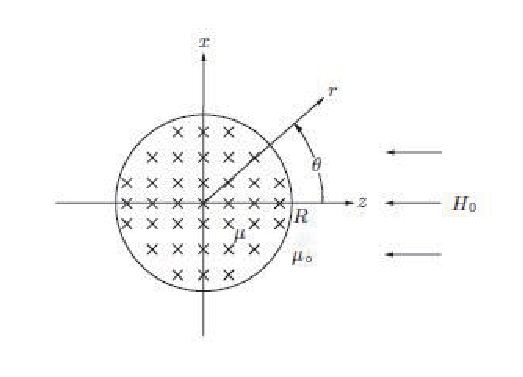
\includegraphics[scale=0.8]{chpt2/figs/fig2.1.eps}
  \caption{均匀场中的磁性球}
\end{figure}

\subsubsection*{问题2.1之解答}
a) 本题用标量势来解是最简单的。磁标量势表示为
$$\vec{H}=-\nabla \phi \eqno (S1.1)$$

对线性、各向同性介质,磁场和磁感应强度的关系为
$$\vec{B}=\mu \vec{H} \eqno (S1.2)$$

问题可以分为两个区域:区域1($r\ge R$)和区域2($r\le R$)。因为在$r=\infty$时,$H_\infty=H_0$,
在$r=0$时,$H\neq \pm \infty$,每个区域的标量势可选为:
$$\phi_1=H_0 r\cos\theta+\frac{A}{r^2}\cos\theta$$
$$\phi_2=C r \cos\theta \eqno (S1.3)$$

注意到,在$r\rightarrow \infty$时,$\phi_1\rightarrow H_0 r \cos\theta$;在$r=0$时,$\phi_2$是有限的。
应用$\nabla$算符,有:
$$\vec{H}_1= H_0(−\cos\theta\vec{i_r} + \sin\theta\vec{i}_\theta) + \frac{A}{r^3}(2 \cos\theta\vec{i_r} + \sin\theta\vec{i_\theta})$$
$$\vec{H}_2=C(-\cos\theta\vec{i_r} + \sin\theta\vec{i}_\theta) \eqno (S1.4)$$

\textbf{边界条件}

1)在$r=R$处,$\vec{H}$的切向分量连续,故无表面电流。这等价于在$r=R$时,有$\phi_1=\phi_2$:
$$H_0 + \frac{A}{R^3} = C \eqno (S1.5)$$

2)在$r=R$处,$\vec{B}$的法向连续:
$$\mu_0\left(-H_0 + 2\frac{A}{R^3} \right)= -\mu C \eqno (S1.6)$$

从S1.5和S1.6式,解出A和C两个常数:
$$C =\frac{3H_0\mu_0}{2\mu_0+\mu}\eqno (S1.7)$$
$$A=(C-H_0)R^3=H_0\left(\frac{\mu_0-\mu}{2\mu_0+\mu}\right)R^3 \eqno (S1.8)$$

于是,$\vec{B}_1$和$\vec{B}_2$可写为:
$$\vec{B}_1= \mu_0 H_0(−\cos\theta\vec{i_r} + \sin\theta\vec{i_\theta}) +
\mu_0\left(\frac{\mu_0-\mu}{2\mu_0+\mu}\right)H_0(\frac{R}{r})^3(2 \cos\theta\vec{i_r} + \sin\theta\vec{i_\theta})$$
$$\vec{B}_2=\frac{3\mu_0\mu H_0}{2\mu_0+\mu}(-\cos\theta\vec{i_r} + \sin\theta\vec{i_\theta}))$$

下面,我们考虑三种$\mu/mu_0$的三种特例。

\textbf{特例1:$\mu/\mu_0=0$}

将$\mu=0$代入2.41式,可得
$$\vec{B}_1= \mu_0 H_0(−\cos\theta\vec{i_r} + \sin\theta\vec{i_\theta}) +
\frac{\mu_0 H_0}{2}(\frac{R}{r})^3 (2 \cos\theta\vec{i_r} + \sin\theta\vec{i_\theta})$$
$$\vec{B}_2=0 \eqno (S1.9)$$

这个球像第I类超导体。球内不允许有磁通密度存在(Meissner效应)。问题2.2将会讨论到,$\vec{H}$在
$r=R$处的$\theta$分量不连续将要求存在表面电流(被限制在一个薄层内)。因为这个电流一旦建立起来,
会一直流下去,这就表明了球对电流是无电阻的。如第一章所言的,存在Meissner效应的材料必须同时是理想导体:
那这种材料其实就是超导体。

\textbf{特例2:$\mu/\mu_0=1$}

这时问题退化为平凡解,即等价于没有球的存在。代入2.41,两个方程将变成同一个。

\textbf{特例3:$\mu/\mu_0=\infty$}

这时表示的是一个理想铁磁材料。软铁的性质与此接近。磁场被“吸”如球内,代入2.41中,有
$$\vec{B}_1= \mu_0 H_0(−\cos\theta\vec{i_r} + \sin\theta\vec{i_theta}) -
\mu_0 H_0\frac{R}{r})^3 (2 \cos\theta\vec{i_r} + \sin\theta\vec{i_theta})$$
$$\vec{B}_2=3\mu_0 H_0(−\cos\theta\vec{i_r} + \sin\theta\vec{i_theta}) \eqno (S1.10)$$

可见,球内的磁感应强度是外施磁场的3倍。注意到,如果球存在磁化饱和,则$\mu$不再是$\infty$。所有磁性
材料都存在的磁场饱和效应将在问题4中讨论。

b) 图2.2给出了$\mu/\mu_0=0.1$和$\mu/\mu_0=100$两种情况下的磁场线。

\begin{figure}
  \centering
 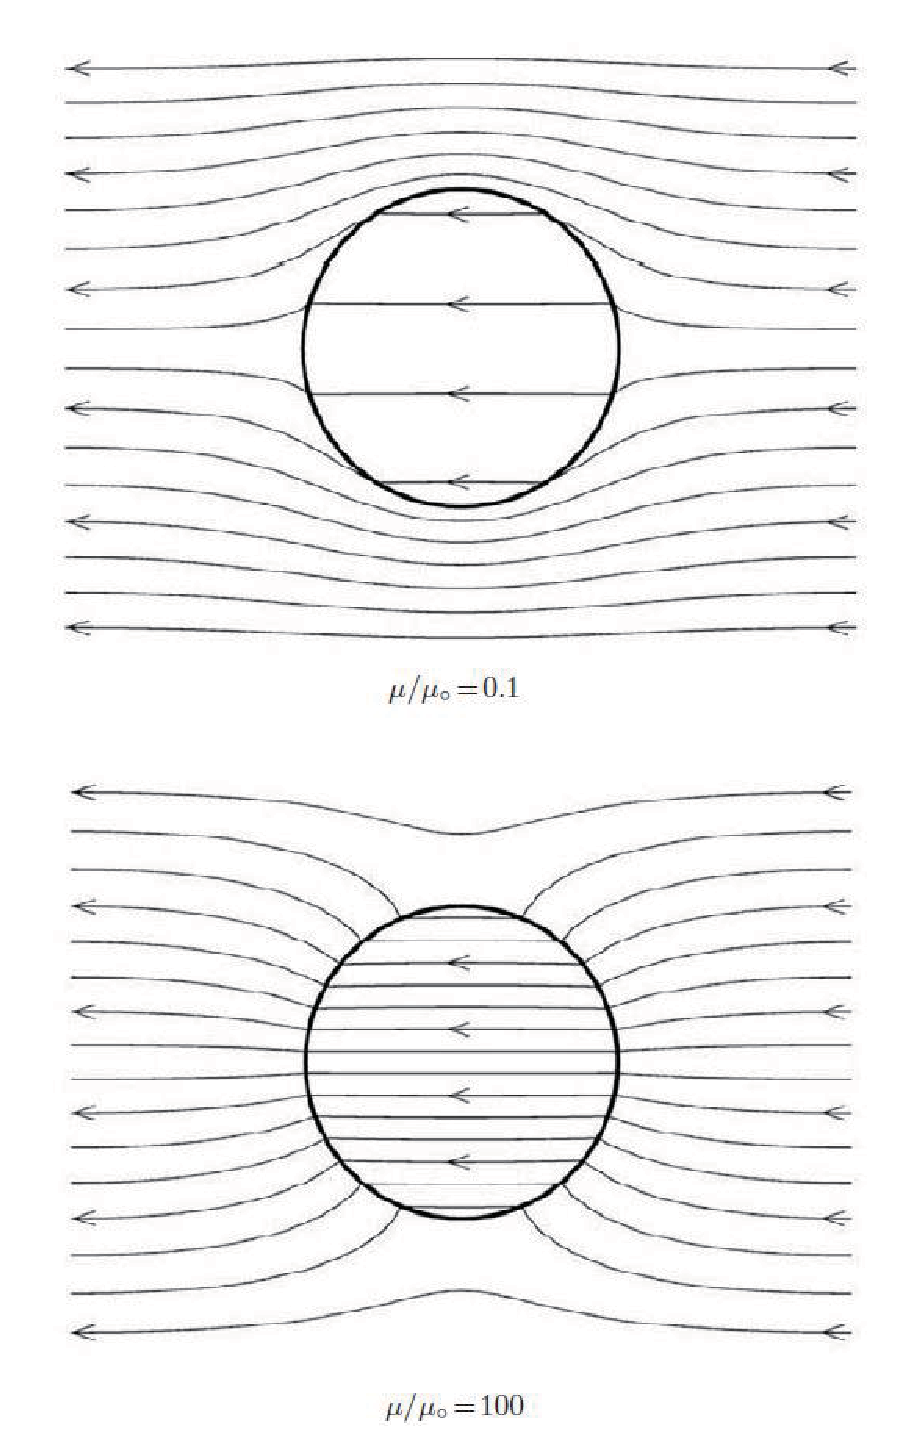
\includegraphics[scale=0.4]{chpt2/figs/fig2.2.eps}
  \caption{两种特例下球内和球附近的磁场线。上球在无穷远处的磁场线密度是球内的2.6倍;下球仅为1.7倍}
\end{figure}

\subsection{问题2.2:均匀场中的第I类超导棒}
本题处理第I代超导体的Meissner效应,并用London超导理论对结果进行解释。
图2.3给出了无限长、圆截面(半径R)的Pb棒,置于垂直于轴向的均匀外磁场中。
\begin{equation*}\label{eqn:2.40}
  \vec{H}_\infty = H_0 (-\cos \theta_{\vec{i_r}}+\sin\theta_{\vec{i_\theta}})
\end{equation*}

式中,$\mu_0H_0=0.08 T$。初始状态,棒处于正常态,于是磁场在棒的内外是处处相同的。棒逐步冷却至超导态。

a)证明在外磁场暂态效应消失后,棒外场的表达式为
\begin{equation}
  \vec{H}_1=H_0(-\cos\theta\vec{i_r}+\sin\theta\vec{i_\theta})+H_0(\frac{R}{r})^2 (\cos\theta\vec{i_r}+\sin\theta\vec{i_\theta})
\end{equation}

b) 证明在穿透深度$\lambda\\ll R$内的电流密度$K_f [A/m]$的表达式为
\begin{equation}
  \vec{K}_f=2H_0 \sin\theta\vec{i_z}
\end{equation}

c)将表面电流密度幅值转换为(体)电流密度$J_f [A/m^2]$。证明用London超导理论导出的电流密度值和这个值是一致的。

\begin{figure}
	\centering
	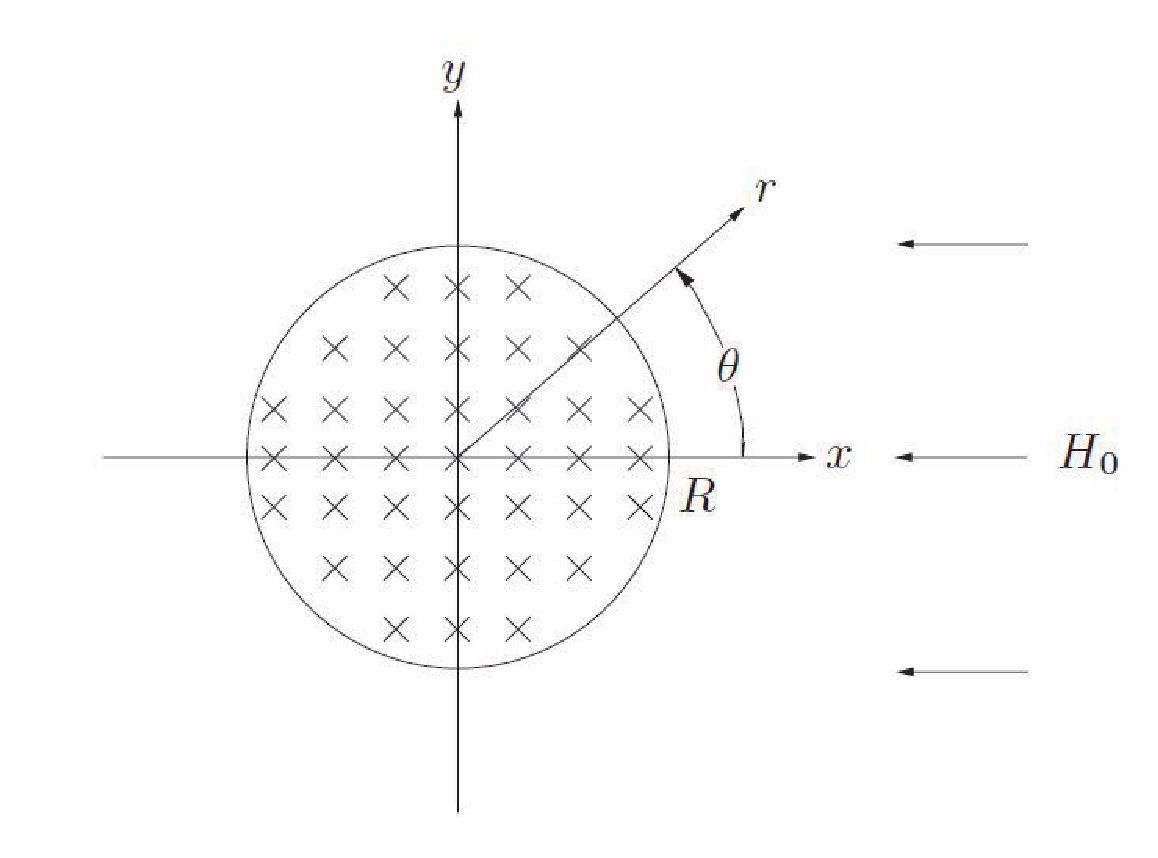
\includegraphics[scale=0.4]{chpt2/figs/fig2.3.eps}
	\caption{无限长、圆截面超导棒置于均匀磁场中}
\end{figure}

\subsubsection*{问题2.2之解答}
a) 问题可以分为两个区域:区域1($r\ge R$)和区域2($r\le R$)。因为我们处理的是第I类超导体,也即圆棒超导时有$\vec{B}_2=0 (\phi_2=0)$。
区域1的场可由势函数导出:
$$  \phi_2=H_0 r \cos \theta +\frac{A}{r} \cos \theta \eqno(S2.1)$$
注意到,当$r\rightarrow \infty $时,$\phi_1\rightarrow H_0 r \cos\theta$。

在圆柱坐标系下使用$\nabla$算符,可以得到$\vec{H}$:
$$\vec{H}_1=-\frac{\partial}{\partial r}(H_0 r \cos\theta +\frac{A}{r}\cos\theta)\vec{i}_r-\frac{1}{r}\frac{\partial}{\partial \theta}(H_0 r \cos\theta +\frac{A}{r}\cos\theta)\vec{i}_\theta \eqno(S2.2)$$
$$=-(H_0 \cos\theta +\frac{A}{r^2}\cos\theta)\vec{i}_r-(-H_0 \sin\theta -\frac{A}{r^2}\sin\theta)\vec{i}_\theta (S2.3)$$
整理S2.3式,可得
$$\vec{H}_1=H_0(-\cos \theta \vec{i}_r+\sin \theta \vec{i}_\theta) +\frac{A}{r^2}(\cos\theta \vec{i}_r+\sin\theta \vec{i}_\theta ) (S2.4)$$
B法向分量的连续性要求S2.3中$\vec{i}_r$的系数在$r=R$处为零:
$$-H_0+\frac{A}{R^2}=0  (S2.5)$$
解出上式,得
$$A=R^2 H_0 (S2.6)$$
于是,超导圆棒外的场(区域1)可以写为:
$$\vec{H}_1=H_0(-\cos \theta \vec{i}_r+\sin \theta \vec{i}_\theta) +H_0 (\frac{R}{r})^2(\cos\theta \vec{i}_r+\sin\theta \vec{i}_\theta ) (2.42)$$

注意到,在$r=R,\theta=90^\circ$时,$|\vec{H}_1|=2H_0$;也即此处的幅值是远场的两倍。物理上看,圆棒处于正常态时场本是在其内部的,进入超导态后,场被“推”出,挤压在$\theta=90^\circ$附近。


b) 因为$2H_0\sin \theta$中的$\vec{H}$在$r=R$处的切向分量不连续,所以肯定存在表面电流密度$\vec{K}_f$流过超导棒。我们有:

\begin{equation}
  \vec{K}_f=\vec{i}_r \times 2H_0\sin\theta \vec{i}_\theta=2H_0\sin\theta\vec{i}_z
\end{equation}

这个正弦电流分布式高能物理设施中被称为“核粒子加速器”内所用的大多数双极磁体的基础。


c) 根据超导电性的London理论,第I类超导体的超导电流密度$J_s$由$J_s=en_{se}v$给出。其中,$e$是电荷量($e=1.6\times 10^{-19}C$),$n_{se}$是超导电子的密度,$v$是超导电子的漂移速度。
超导电子的密度\textbf{大致}上等于自由电子的密度:

\begin{equation}
n_{se}\simeq n_{fe}=\frac{\rho N_A}{W_A}
\end{equation}

对于铅,$\rho=11.4 g/cm^3,N_A=6.023\times 10^{23},W_A=207.2 g/mole$,我们得到单位体积的电子数量:
$$
n_{se}=\frac{11.4\times 6.023\times 10^{23}}{207.2} \simeq 3.3\times 10^{28}
$$
超导电子的漂移速度约为$200m/s$,于是我们可以得到$J_s$的量级:
$$
J_s=e n_{se} v\sim 1.6\times 10^{-19} \times 3.3\times 10^{28} \times 200 \sim 1\times 10^{12} A/m^2
$$
在上述铅圆柱棒所要求的表面电流密度($K_f=J_f \lambda$)下,$J_f$应\textbf{大致}上与$J_s$相等,也即与上面所计算的$J_s$在同一个量级上。
London理论给出了供超导电流流过的超导体表面穿透深度$\lambda$的表达式:
$$
\lambda=\sqrt{\frac{m}{\mu_0 e^2 n_{se}}}
$$
其中,$n_{se}$上面已经给出,$m=9.1\times 10^{-31} kg$,则:
$$
\lambda=\sqrt{\frac{9.1\times 10^{-31}}{4\pi \times 10^{-7}\times 1.6\times 10^{-19}\times 3.3\times 10^{28}}}\simeq 3\times 10^{-8} m
$$
由于$K_f=J_f\lambda$,则
$$
J_f=\frac{2H_0}{\lambda}=\frac{2\mu_0 H_0}{\mu_0 \lambda}\simeq 4\times 10^{12} A/m^2
$$
也即,$J_f$与$J_s$\textbf{大致}上相等。


\subsection{讨论2.1:均匀场中的理想导体球}
本题我们推导理想导体($\rho=0$)球置于磁场中的定量磁场表达。特别是针对图 1.1c中的$C\Rightarrow D$转变过程。
点C处,包括球内的整个空间处于均匀外场中(问题1,eq. 2.40)。外施场合问题1中的图 2.1相同。

当均匀外场降至$0$(图1.1c中的D点),由于球内的磁感应无法改变,其磁场$\vec{H_2}$必保持不变。
$$
\vec{H_2}=H_0 (-\cos\theta \vec{i_r}+\sin\theta \vec{i_\theta})  (r\le R)
$$

远离球中心($r\rightarrow \infty$)处的外场$\vec{H_1}$为0。靠近球处的磁场可由标量势$\phi_1=(A/r^2)\cos\theta$导出。
在$\phi_1$上应用$\nabla$算符,可得到球坐标下的偶极场:
$$
\vec{H_1}=\frac{A}{r^3}(2\cos\theta \vec{i_r}+\sin\theta \vec{i_\theta})  (r\ge R)
$$

在$r=R$处,$B$的法向分量应连续。由于在$\theta=0$处球内外的磁场均仅有法向分量,故:
$$
-H_0=2\frac{A}{R^3}
$$

于是,$A=-\frac{H_0 R^3}{2}$,进而
$$
\vec{H_1}=-H_0(\frac{R}{r})^3 (\cos\theta \vec{i_r}+\frac{1}{2}\sin\theta \vec{i_\theta})
$$

上式即磁场分布的定量表达。不同的是,图1.1c的外场是自下向上的,而图2.1的磁场是自右向左的。

在$r=R$处,磁场切向分量的不连续等于在$r=R$处球表面电流密度$\vec{K_f}$。联立方程2.6以及上面3式,有
\begin{equation}
  \vec{K_f}=\vec{i_r}\times [H_0 \sin\theta \vec{i_\theta}-(-\frac{1}{2}H_0 \sin\theta \vec{i_\theta})]=\frac{3}{2}H_0\sin\theta\vec{i_\theta}
\end{equation}

值得一提的是,这个$\sin\theta$分布,可以用一个绕在球上的在z轴均匀匝密度的“薄”线圈来近似。


\subsection{问题2.3:球壳的磁屏蔽}
本问题处理被动磁屏蔽。在MRI、磁悬浮等一些人和磁场敏感设备必须暴露于磁场外缘的高场系统中磁屏蔽是非常重要的课题。
美国食药局(FDA)规定,MRI中的最大外缘磁场为5高斯($0.5mT$)。

在空间中的球星区域,屏蔽一个均匀磁场$\vec{H}_\infty$:
$$
\vec{H}_\infty=H_0 (-\cos\theta \vec{i_r}+\sin\theta \vec{i_\theta})
$$

为了形成屏蔽,可以用一个外径为$2R$、壁厚$d/R\ll 1$、高磁导率材料($\mu/\mu_0 \gg 1$)的球壳,如图2.4所示。

a) 将本问题视为均匀外磁场中的磁性球壳。证明$H_{ss}/H_0$有如下表达式。其中,$H_{ss}$为球壳内($r\le R-d$)的磁场幅值
\begin{equation}
\frac{H_{ss}}{H_0}=\frac{9\mu_0 \mu}{9\mu_0 \mu+2(\mu-\mu_0)^2\left[1-\left(1-\frac{d}{R}\right)^3\right]}
\end{equation}

b)证明,在极限情况$\mu/\mu_0\gg 1$和$d/R\ll 1$下,$H_{ss}/H_0$可约化为
\begin{equation}
\frac{H_{ss}}{H_0}\simeq \frac{3}{2}(\frac{\mu_0}{\mu})(\frac{R}{d})
\end{equation}

c)用微扰法得到上式。首先,在$\mu=\infty$条件下解出壳上($R-d\le r\le R$)的磁场。接着,用微扰法在$\mu/\mu_0 \gg 1$条件下得到上式。

d)实践中,屏蔽材料中的磁通必须控制在材料的饱和磁通($\mu_0 M_{sa}$)之下。证明,可保持壳不饱和的$d/R$表达式为
\begin{equation}
\frac{d}{R} \ge \frac{3H_0}{2M_{sa}}
\end{equation}

e)画出$\mu/\mu_0 \gg 1$情况下的场线。

\begin{figure}
  \centering
 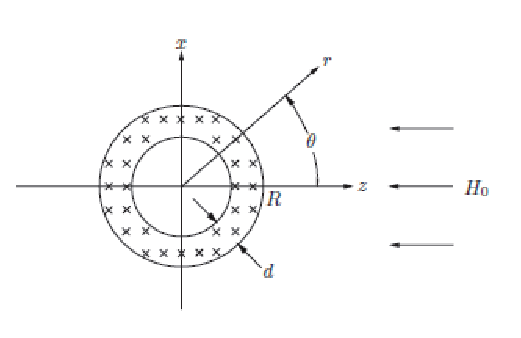
\includegraphics[scale=0.9]{chpt2/figs/fig2.4.eps}
  \caption{均匀磁场中的磁性球壳}
\end{figure}

\subsubsection*{问题2.3之解答}
a)问题可以分为三个区域:区域1($r\ge R$);区域2(球壳);区域3($r\le R-d$)。相应的势函数为:
\begin{eqnarray*}
% \nonumber % Remove numbering (before each equation)
  \phi_1 &=& H_0 r\cos\theta+\frac{A}{r^2}\cos\theta \\
  \phi_2 &=& C r \cos\theta+\frac{D}{r^2}\cos\theta \\
  \phi_3 &=& H_{ss} r\cos\theta
\end{eqnarray*}

注意到,在$r\rightarrow \infty$时,$\phi_1 \rightarrow H_0 r\cos\theta$以及在$r\rightarrow 0$时,$\phi_3$为有限值。应用球坐标下的$\nabla$算符,得到
\begin{eqnarray*}
% \nonumber % Remove numbering (before each equation)
  \vec{H}_1 &=& H_0 (-\cos\theta\vec{i_r}+\sin\theta\vec{i}_\theta)+\frac{A}{r^3} (2\cos\theta\vec{i_r}+\sin\theta\vec{i}_\theta)\\
  \vec{H}_2 &=& C(-\cos\theta\vec{i_r}+\sin\theta\vec{i}_\theta)+\frac{D}{r^3} (2\cos\theta\vec{i_r}+\sin\theta\vec{i}_\theta)\\
   \vec{H}_3 &=& H_{ss}  (-\cos\theta\vec{i_r}+\sin\theta\vec{i}_\theta)
\end{eqnarray*}

边界条件为:
\begin{enumerate}
  \item $r=R$处,$\vec{H}$的切向分量$H_\theta$连续:$\phi_1=\phi_2   $
  \item 类似的,在$r=R-d$处,$H_\theta$连续:$\phi_2=\phi_3  $
  \item 在$r=R$处,$\vec{B}$的法向分量$B_r$连续
  \item 类似的,在$r=R-d$处,$B_r$连续
\end{enumerate}

由上述边界条件,可导出下面的四个方程:
\begin{eqnarray*}
% \nonumber % Remove numbering (before each equation)
  H_0+\frac{A}{R^3}&=& C+\frac{D}{R^3} \\
  C+\frac{D}{(R-d)^3}&=& H_{ss}\\
  \mu_0(-H_0+\frac{2A}{R^3})&=& \mu(-C+\frac{2D}{R^3})\\
  \mu[-C+\frac{2D}{(R-d)^3}&=& -\mu_0 H_{ss}
\end{eqnarray*}

联立1、2式,消去C:
$$
\frac{A}{R^3}+D[\frac{1}{(R-d)^3}-\frac{1}{R^3}]-H_ss =-H_0
$$

联立2、4式,解出D:
$$
D=\frac{\mu-\mu_0}{2\mu} (R-d)^3 H_ss
$$

于是,可以$H_{ss}$表示$A/R^3$:
$$
\frac{A}{R^3}=H_{ss}\{1-\frac{\mu-\mu_0}{3\mu}[1-(1-\frac{d}{R})^3]\}-H_0
$$

联立3、4式,得到:
$$
\frac{2A}{R^3}+2\frac{\mu}{\mu_0}D[\frac{1}{(R-d)^3}-\frac{1}{R^3}]+H_ss =H_0
$$

于是,可以得到
\begin{equation*}
\frac{H_{ss}}{H_0}=\frac{9\mu_0 \mu}{9\mu_0 \mu+2(\mu-\mu_0)^2\left[1-\left(1-\frac{d}{R}\right)^3\right]}
\end{equation*}

b) 方程右侧的分子分母同除$\mu_0^2$,应用极限$\mu/\mu_0)\gg 1$和$d/R\ll 1$:
$$\frac{H_{ss}}{H_0}\simeq \frac{9\mu/mu_0}{9\frac{\mu}{\mu_0}+2(\frac{\mu}{\mu_0})^2[1-(1-3\frac{d}{R})]}$$
$$\simeq\frac{3}{3+2(\frac{\mu}{\mu_0})(\frac{d}{R})}$$

在$\mu d/\mu_0 R \gg 1$的特殊情况下,上式可以进一步简化为:
$$\frac{H_{ss}}{H_0}\simeq \frac{2}{3}(\frac{\mu_0}{\mu})(\frac{R}{d})$$

c)我们假设$\mu$为无限大。这要求B线在$r=R$处垂直于球壳。这是因为在$r=R$处,$\vec{H}_1$仅有径向分量。由于壳内$H=0$,故在$r=R$处$H_\theta$必须连续。
注意到,当$\mu=\infty$时,$C=D=0$。这样,$A=-R^3 H_0$,于是在$r=R$处
$$\vec{H}_1=-3 H_0 \cos\theta \vec{i_r}$$

\begin{figure}
	\centering
	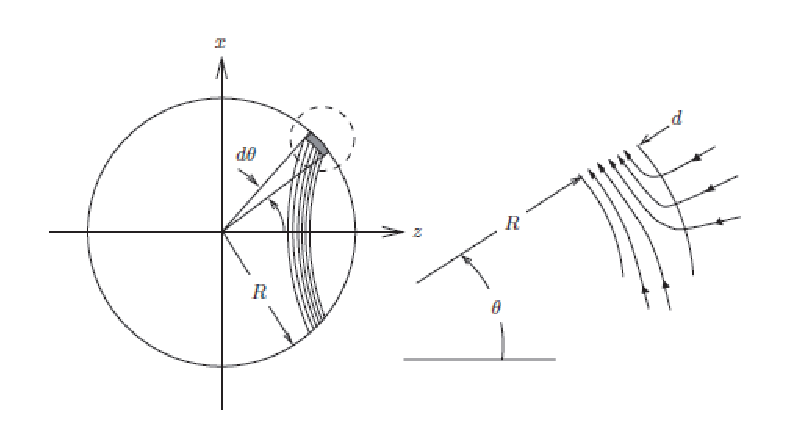
\includegraphics[scale=0.7]{chpt2/figs/fig2.5.eps}
	\caption{通过球壳$\pm \theta$边界内区域进入壳的磁通}
\end{figure}

B线局限在壳内,不会“逸”至区域3。也即,壳内的B仅有$\vec{i}_\theta$分量。应用磁通连续性($\nabla \cdot \vec{B}=0$)并在$\mu=\infty$条件下解$B_2$。解出$B_2$
后,可以得到$\mu \neq \infty$但$\mu/\mu_0 \gg 1$时$\vec{H}_3$的近似表达式。

首先,计算通过表面区域$\pm \theta$边界内进入壳的总磁通(图2.5)。根据图中的微元积分
$$
\Phi=\mu_0\int_{0}^{\theta} \vec{H}_1 \cdot d\vec{A}=\mu_0\int_{0}^{\theta} 3H_0\cos\theta 2\pi R^2 \sin\theta d\theta=3\pi\mu_0 R^2 H_0 \sin^2 \theta
$$

这个$\Phi$一定等于在球壳$\theta$处$\theta$方向的磁通量。
在$d\ll R$条件下,壳在$\theta$处的截面区域$A_2$可由下式给出
$$
A_2\simeq d\cdot 2\pi R\sin\theta
$$

我们有
$$\Phi=3\pi\mu_0 R^2 H_0 \sin^2 \theta\simeq B_2 A_2=B_2 d 2 \pi R \sin\theta$$

解出$B_2$,得
$$
\vec{B}_2\simeq \frac{3}{2}\mu_0 (\frac{R}{d}) H_0\sin\theta\vec{i}_\theta
$$

注意到上式的$\vec{B}_2$是在$\mu=\infty$条件下得到的。现在我们可以导出$\vec{H}_3$的近似表达。
由于$\vec{H}$的$\vec{i}_\theta$分量在$r=R-d$处必须连续,于是
$$
H_{\theta 3}\simeq \frac{B_{\theta 2}}{\mu}=\frac{3}{2}(\frac{\mu_0}{\mu})(\frac{R}{d})H_0\sin\theta
$$

得到了$H_{\theta 3}$,我们就可以给出$\vec{H}_3$的完整表达式了:
$$
\vec{H}_3\simeq \frac{B_{\theta 2}}{\mu}=\frac{3}{2}(\frac{\mu_0}{\mu})(\frac{R}{d})H_0(-\cos\theta\vec{i_r}+\sin\theta\vec{i}_\theta)
$$

于是
$$\left|\frac{\vec{H}_3}{H_0}\right|\simeq \frac{3}{2}(\frac{\mu_0}{\mu})(\frac{R}{d})$$

注意:此处的微扰法需要$\mu=\infty$和$d\ll R$条件,但无需$\mu d/\mu_0 R \gg 1$条件。

d)应当明确,不能为了满足$d/R \ll 1$而将d选的特别小。事实上,下面的分析仅在下式条件满足时有效:
$$
\frac{\mu_0}{\mu} \ll \frac{d}{R} \ll 1
$$

实际的$\mu$不可能无限大。屏蔽材料会随着外场的增大最终饱和。因此,壳内的最大磁通(在$\theta=90\circ C$时取得)必须小于屏蔽壳材料的饱和磁通$\mu_0 M_{sa}$。
于是
$$
\frac{3}{2}(\frac{R}{d})\mu_0 H_0 \le \mu_0 M_{sa}
$$

解出$d/R$,有
$$\frac{d}{R}\gg \frac{3H_0}{2M_{sa}}$$

表\ref{my-label} 给出了三种材料的微分$\mu/\mu_0$和$\mu_0M(H_0)$的近似值。其中,$(\mu/\mu_0)_{dif}\equiv \Delta M/ \Delta H_0 |_{\mu_0 H_0}$,$\mu_0 H_0$的范围为$0\sim 1000$高斯。
后面还给出了这三种材料的饱和磁通值。这几种材料常用来屏蔽$\sim 100$高斯下的磁场。

\begin{table}[]
\centering
\caption{几种材料的屏蔽特征值}
\label{my-label}
\begin{tabular}{|c|c|c|c|c|c|c|}
\hline
\multirow{2}{*}{$\mu_0 H_0$[gauss]} & \multicolumn{2}{c|}{annealed ingot iron} & \multicolumn{2}{c|}{As-Cast Steel} & \multicolumn{2}{c|}{Vanadium Permendur} \\ \cline{2-7}
                                  &$ (\mu/mu_0)_{dif} $      & $\mu_0 $M[T]  & $(\mu/mu_0)_{dif}   $ &$ \mu_0 M$[T]   &$ (\mu/mu_0)_{dif}    $  & $\mu_0 M$[T]      \\ \hline
1                                 & 7710                   & 0.375           & na                  & na           & na                    & na              \\ \hline
3                                 & 3850                   & 0.91            & 1660                & 0.25         & 4845                  & 0.65            \\ \hline
5                                 & 500                    & 1.42            & 1155                & 0.51         & 1875                  & 1.25            \\ \hline
10                                & 115                    & 1.54            & 565                 & 0.93         & 545                   & 1.67            \\ \hline
20                                & 47                     & 1.60            & 180                 & 1.25         & 170                   & 1.96            \\ \hline
50                                & 23.5                   & 1.70            & 50                  & 1.52         & 17                    & 2.10            \\ \hline
100                               & 17.5                   & 1.81            & 25                  & 1.70         & 4.8                   & 2.15            \\ \hline
200                               & 8.25                   & 1.93            & 10                  & 1.85         & 1.3                   & 2.17            \\ \hline
500                               & 2.0                    & 2.05            & 1.0                 & 1.92         & 0.26                  & 2.18            \\ \hline
1000                              & 0.4                    & 2.11            & 0.45                & 2.01         & 0.07                  & 2.19            \\ \hline
$\mu_0 M_{sa} $                     & \multicolumn{2}{c|}{2.13[T]}             & \multicolumn{2}{c|}{2.03[T]}       & \multicolumn{2}{c|}{2.20[T]}            \\ \hline
\end{tabular}
\end{table}

e) $\mu/\mu_0=100$磁性球壳置于均匀场中的磁场分布如图2.6所示。

\begin{figure}
  \centering
 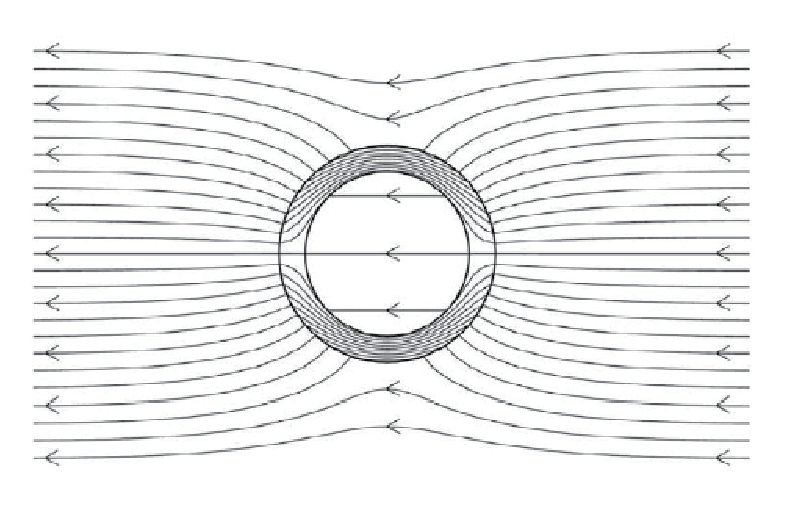
\includegraphics[scale=0.7]{chpt2/figs/fig2.6.eps}
  \caption{$\mu/\mu_0=100$磁性球壳置于均匀场中的磁场分布。注意到进出球壳的磁场线是近乎垂直于壳的。}
\end{figure}

\subsection{讨论2.2:用圆柱壳屏蔽}
我们用类似于问题4中所用的微扰技术推导$H_{cs}/H_0$的表达式。式中,$H_{cs}$是置于均匀外场采用高磁导率($\mu/\mu_0 \gg 1$)材料的圆柱壳($d/R\ll 1$)内部($r\le R-d$)的磁场的幅值。
在二维柱坐标系下,外场有如下形式:
$$
\vec{H}_\infty =H_0 (-\cos\theta \vec{i_r}+\sin\theta\vec{i}_\theta)
$$

我们假定圆柱材料的$\mu$是无限大的,这样B线在$r=R$处必须垂直于圆柱。于是,在$r=R$处,有
$$\vec{H}_1 =-2 H_0 \cos\theta \vec{i_r}$$

当然,壳内的B是$\theta$方向的。在$d/R\ll 1$条件下,磁通连续性要求B满足:
$$B_2 d=\int_{0}^{\theta}2\mu_0 H_0 R\cos\theta d\theta=2\mu_0 R H_0 \sin\theta$$

于是,
$$\vec{B}_2=2\mu_0 (\frac{R}{d})H_0 \sin\theta \vec{i}_\theta$$

已知$\mu=\infty$下的$\vec{B}_2$,我们可以得到$\mu/\mu_0 \gg 1$下的$\vec{H}_2$:
$$\vec{H}_2= \frac{\vec{B}_2}{\mu}\simeq 2(\frac{\mu_0}{\mu}) (\frac{R}{d})H_0 \sin\theta \vec{i}_\theta$$

因为在没有表面电流时$H_\theta$是连续的,区域2和区域3一定有$H_{\theta 2}=H_{\theta 3}$。于是,在$r=R-d$处:
$$H_{\theta 3}=H_{\theta 2}\simeq 2(\frac{\mu_0}{\mu}) (\frac{R}{d})H_0 \sin\theta$$

从上面的表达式,可以得出:
$$\vec{H}_3 \simeq 2(\frac{\mu_0}{\mu}) (\frac{R}{d})H_0 (-\cos\theta \vec{i_r}+\sin\theta\vec{i}_\theta)$$
$$\left|\frac{\vec{H}_3}{H_0}\right|\equiv\frac{H_{cs}}{H_0}\simeq 2(\frac{\mu_0}{\mu}) (\frac{R}{d})$$

如问题4中的球壳一样,圆柱壳的厚度也不能无线薄。它必须有保持足够的厚度以防止饱和:
$$\mu H_{cs}=2\mu_0 H_0 \frac{R}{d}\le \mu_0 M_{sa}$$

也即
$$\frac{d}{R}\ge \frac{2H_0}{M_{sa}}$$


\subsection{问题2.4:四个偶极子簇的远场}
本题讨论如下图布置的四个理想偶极子簇的远场。各偶极子的方向如图箭头所示。两个相反偶极子的中心距为$2\delta_d$。各偶极子j均为零绕组厚度,直径均为$2r_d$,在y向的总长度为$l_d$,距离偶极子径向($r_j$)位置的远场($r_j \gg l_d$)可建模为球偶极子场$\vec{B}_j$:
$$\vec{B}_j=\frac{r_d^2 l_d B_0}{2r_j^3}(\cos\theta_j \vec{i}_{r_j}+\frac{1}{2} \sin\theta_j \vec{i}_{\theta_j})$$

式中,$r_j$is measured from the center of each dipole and $\theta_j$ in each dipole is defined such that the field inside the winding points in the $r_j$-direction when $\theta_j=0$。图2.7给出了各偶极子内场的方向,还定义了对所有偶极子共同的$r-\theta$坐标系和$z-x$坐标系。注意到,$r\gg \delta_d$,我们有$\mathscr{\theta}_1=\theta+180^\circ,\theta_2=\theta-90^\circ,\theta_3=\theta,\theta_4=\theta + 90^\circ$。

证明,忽略各偶极子的末端效应,仅考虑$y=0$平面,本组合系统的远场($r/\delta_d \gg 1$)近似表达式为:
$$ \vec{B}\simeq \frac{3r_d^2 l_d B_0 \delta_d}{r^4}(-\sin 2\theta \vec{i}_r+\frac{1}{2}\cos 2\theta \vec{i}_\theta)$$

\begin{figure}
  \centering
 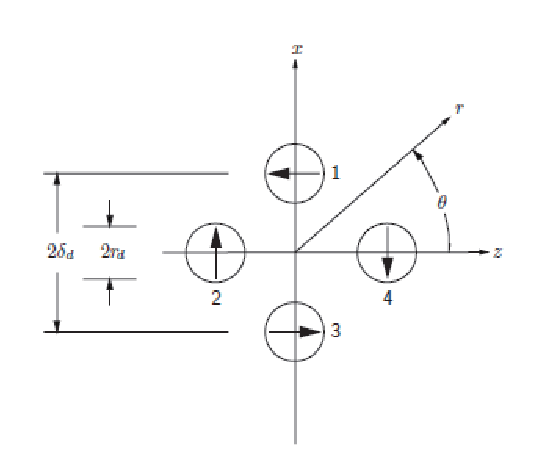
\includegraphics[scale=0.8]{chpt2/figs/fig2.7.eps}
  \caption{四个偶极子布置的横截面。每个偶极子的箭头指示线圈内场的方向。}
\end{figure}


\subsubsection*{问题2.4之解}
对于$r\gg \delta_d$,每个偶极子的$r_j$可以用$r$和$\theta$表示:
$$r_1\simeq r-\delta_d \sin\theta$$
$$r_2\simeq r+\delta_d \cos\theta$$
$$r_3\simeq r+\delta_d \sin\theta$$
$$r_4\simeq r-\delta_d \cos\theta$$

由此,可以得到各偶极子采用$\theta$表示的场:
$$ \vec{B}_1 \simeq \frac{r_d^2 l_d B_0}{2(r-\delta_d\sin\theta)^3}(-\cos\theta \vec{i}_r-\frac{1}{2}\sin\theta \vec{i}_\theta)$$
$$ \vec{B}_2 \simeq \frac{r_d^2 l_d B_0}{2(r+\delta_d\cos\theta)^3}(\sin\theta \vec{i}_r-\frac{1}{2}\cos\theta \vec{i}_\theta)$$
$$ \vec{B}_3 \simeq \frac{r_d^2 l_d B_0}{2(r+\delta_d\sin\theta)^3}(\cos\theta \vec{i}_r+\frac{1}{2}\sin\theta \vec{i}_\theta)$$
$$ \vec{B}_4 \simeq \frac{r_d^2 l_d B_0}{2(r-\delta_d\cos\theta)^3}(-\sin\theta \vec{i}_r+\frac{1}{2}\cos\theta \vec{i}_\theta)$$

对于$r\gg \delta_d$,各项的分母可对$\delta_d/r$作一阶展开,成为:
$$ \vec{B}_1 \simeq \frac{r_d^2 l_d B_0}{2 r^3}\left[1+3(\frac{\delta_d}{r})\sin\theta \right](-\cos\theta \vec{i}_r-\frac{1}{2}\sin\theta \vec{i}_\theta)$$
$$ \vec{B}_2 \simeq \frac{r_d^2 l_d B_0}{2 r^3}\left[1-3(\frac{\delta_d}{r})\cos\theta \right](\sin\theta \vec{i}_r-\frac{1}{2}\cos\theta \vec{i}_\theta)$$
$$ \vec{B}_3 \simeq \frac{r_d^2 l_d B_0}{2 r^3}\left[1-3(\frac{\delta_d}{r})\sin\theta \right](\cos\theta \vec{i}_r+\frac{1}{2}\sin\theta \vec{i}_\theta)$$
$$ \vec{B}_4 \simeq \frac{r_d^2 l_d B_0}{2 r^3}\left[1+3(\frac{\delta_d}{r})\sin\theta \right](-\sin\theta \vec{i}_r+\frac{1}{2}\cos\theta \vec{i}_\theta)$$

组合上面几式,可以得到
$$ \vec{B}=\vec{B}_1+\vec{B}_2+\vec{B}_3+\vec{B}_4\simeq \frac{3r_d^2 l_d B_0 \delta_d}{r^4}(-\sin 2\theta \vec{i}_r+\frac{1}{2}\cos 2\theta \vec{i}_\theta)$$

注意到,$|B|$按$\propto 1/r^4$衰减而不是像单个偶极子一样的$\propto 1/r^3$衰减。


\subsection{问题2.5:铁电磁体的磁极形状}
图2.8给出了铁制电磁铁的剖面。两个铁磁材料制成的圆柱形磁极相对放置,圆柱尖端倒角成锥形(图中的阴影部分)。
磁极上的线圈(图中未画出)通电后,两极间的间隙内将产生一个相对均匀的磁场。
中心场理论上没有上限,因为它是$\propto \ln(R_2/R_1)$增长的。其中,$R_1$和$R_2$分别是锥体顶部和基部的直径。
由于随着$R_2$增加,磁体的质量会变得很大,所以实践中的中心场上限$\sim 7$T(Bellevue, Paris; Uppsala Uni.,Sweden)。
由于尖端部分的磁矩产生的场对中心的z向场有一个负的贡献,所以,尖角能够加强中心场。

证明:若铁芯在与系统z轴平行方向励磁,$\theta_{tp}=54^\circ 44^\prime$是这种简单磁极几何的最优角度。
假定中心场是均匀分布于磁极件上的磁矩产生的场的叠加。z向励磁的磁矩$\vec{m_A}[A\cdot m^2]$产生的偶极场为:
$$\vec{H}_{m_A}=\frac{\vec{m_A}}{r^3}(\cos\theta \vec{i}_r+\frac{1}{2}\sin\theta\vec{i}_\theta)$$

$\vec{H}_{m_A}(r,\theta)$关于z轴对称,可以从标量势$\cos\theta/r^2$导出。

提示:解出位于磁极倒角基部边缘上(图示)的单个磁矩$m_A \uparrow$在z轴中心的场。

\subsubsection*{问题2.5的解}

$m_A$产生的在中心的场的z向分量$H_{m_A z}$为:
$$H_{m_A z}=\frac{\vec{m_A}}{r^3}(\cos^2\theta-\frac{1}{2}\sin^2\theta)$$

式中,$r_A$是$m_A$距中心的距离。在$\theta=\theta_{tp}$时,上述方程的右侧为0。于是
$$\cos^2\theta_{tp}-\frac{1}{2}\sin^2\theta_{tp}=0$$

于是有$\cos\theta_{tp}=1/\sqrt{3}$或$\tan\theta_{tp}=\sqrt{2}$,也即$\theta_{tp}\simeq 54.736^\circ\simeq54^\circ 44^\prime$。

我们注意到,对阴影区中基线之上的磁矩均有$\theta_{tp}>54^\circ 44^\prime$。由于随$\theta$值的增加,$\cos\theta$递减而$\sin\theta$递增,
在$\theta_{tp}>54^\circ 44^\prime$时,$H_{m_A z}$为负。以$\theta_{tp}=54^\circ 44^\prime$倒角磁极可以消除这种负的贡献,最大化中心场。

值得一提的是,NMR质谱仪中的“神奇角”(magic angle)也是$54^\circ 44^\prime$。通常,NMR样品以这个“神奇角”与主轴场取向放置以减少各向异性的作用。

\begin{figure}
  \centering
 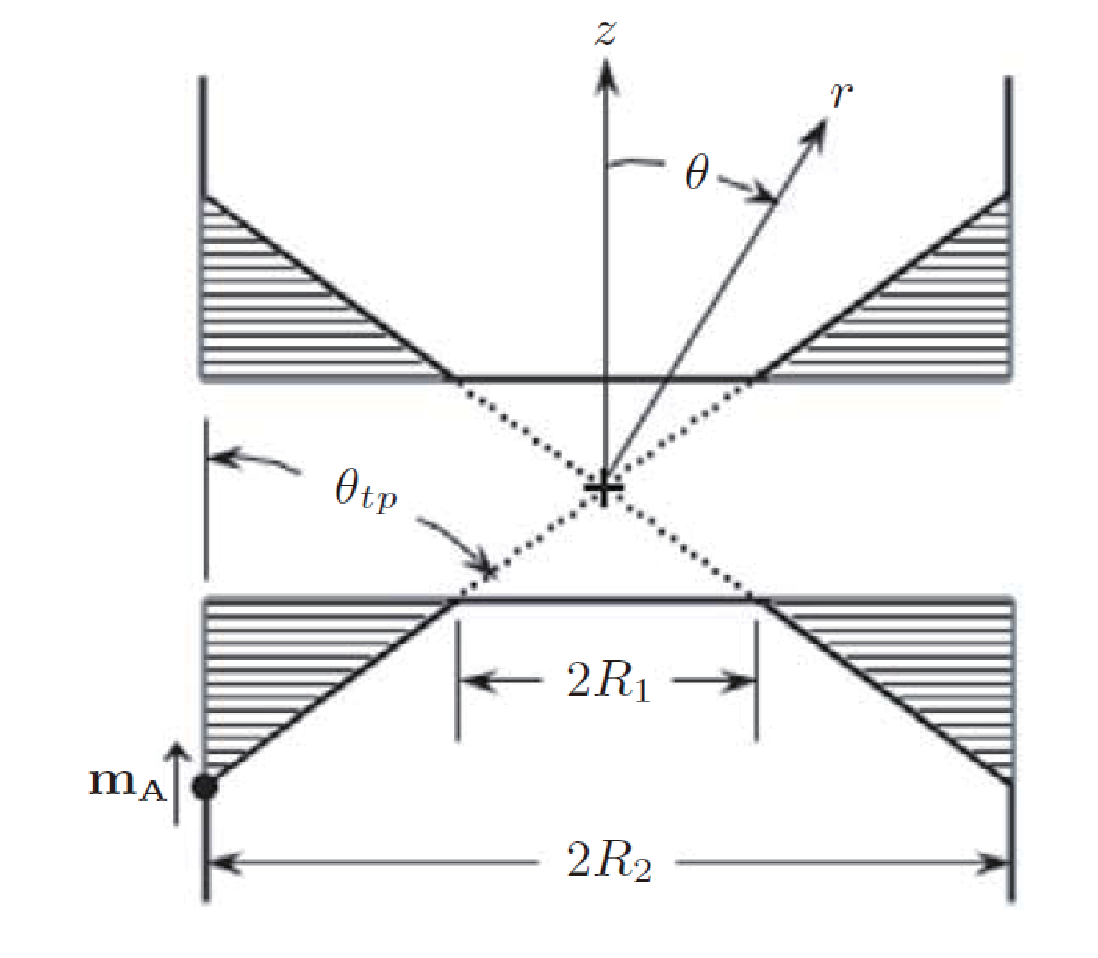
\includegraphics[scale=0.4]{chpt2/figs/fig2.8.eps}
  \caption{电极对,倒角为$\theta_{tp}$。图中$\bullet$指示了磁矩$\vec{m_A}\uparrow$的位置。}
\end{figure}

\subsection{讨论2.3:永磁体}
永磁磁体是日常生活中大量设备如汽车、电视、电脑、手机、冰箱等的关键部件。实际上,如果没有永磁体,今日的现代生活将难以存续。
在低场($<1$)T的MRI中,永磁体是超导体的竞争对手。由于永磁磁体既无需制冷也很便宜,永磁MRI很受欢迎。

表2.6给出了90年(1910s-1990s)间永磁体和超导体的发展。永磁体性能以最大磁能$BH|_{mx}$表示,而超导体以最高临界温度$T_c|_{mx}$表示。
这期间,$BH|_{mx}$提高了约30倍,$T_c|_{mx}$提高了约20倍。

永磁体照这个步调发展下去,在不久的将来,永磁体MRI将能达到$\sim 1$T。
在这个磁场之上,还是超导的天下。

\begin{table}[]
\centering
\caption{永磁体和超导体的发展历程}
\label{磁体和超导体的发展}
\begin{tabular}{|c|c|c|c|c|}
\hline
年代        & 永磁体 & $BH|_{mx}$[$kJ/m^3$] & 超导体 & $T_c|_{mx}$[K]   \\ \hline
1910      &  特种钢   & 11       &  Pb   & 7.2 \\ \hline
1920-1940 &  Alnico 1-4   & 15       &   NbN  & 16  \\ \hline
1950      &   Alnico 5  & 35       &    $Nb_3 Sn$ & 18  \\ \hline
1960      &   Alnico 8,9  & 55       &   $Nb_{12}Al_3 Ge$  &   19  \\ \hline
1970      &   $SmCo_5 $  & 140      &  $Nb_3Ge$   & 23    \\ \hline
1980      &   $Sm(CoCuFeZr)  $& 240      &  $Bi_2 Sr_2 Ca_2 Cu_3 O_x$   & 118 \\ \hline
1990      &  $Nd_2Fe_{14}B$   & 350      & $(Hg, Pb) Sr_2 Ca_2 Cu_3 O_x$    & 133 \\ \hline
\end{tabular}
\end{table}



\subsection{问题2.6:圆柱中的准静态场}
半径为R的长薄圆柱由理想导体($\rho=\infty$,非超导)薄板制成,侧面开有宽$\delta$的窄缝(如图)。
圆柱置于正弦时变磁场中:
$$\vec{H}_\infty(t)=Re[H_0 e^{j\omega t}] \vec{i}_z$$

式中,$H_0$是复幅值。忽略端部效应。

a)忽略$\delta/R$阶项。证明:跨窄缝短边的一阶复电压幅值为:
$$V_{1|0}\equiv V_{1|\theta=0}=-j\omega \pi R^2 \mu_0 H_0$$

b)一个电阻率为$\rho[\Omega\cdot m]$的正常金属板置于窄缝将圆柱开缝恰好连接起来。推导通过该板的一阶复电流密度(轴向单位长度)$J_1 [A/m]$的表达式。
假定:驱动频率($\omega/2\pi$)足够小,磁场仍保持原准静态形式;电流在板截面上均匀流过。

c)在无金属板存在(或$\rho_s=\infty$)条件下,在圆柱腔内画出6条一阶复电场矢量($\vec{E}_1$)线,指明电场的重要特征。

d)在无金属板存在条件下,推导两点间的一阶电压的线积分$V_1 |_{\theta=-\pi/2}^{\theta=+\pi/2}$的表达式,即一点位于$\theta=+\pi/2$,另一点位于$\theta=-\pi/2$。

\begin{figure}
  \centering
 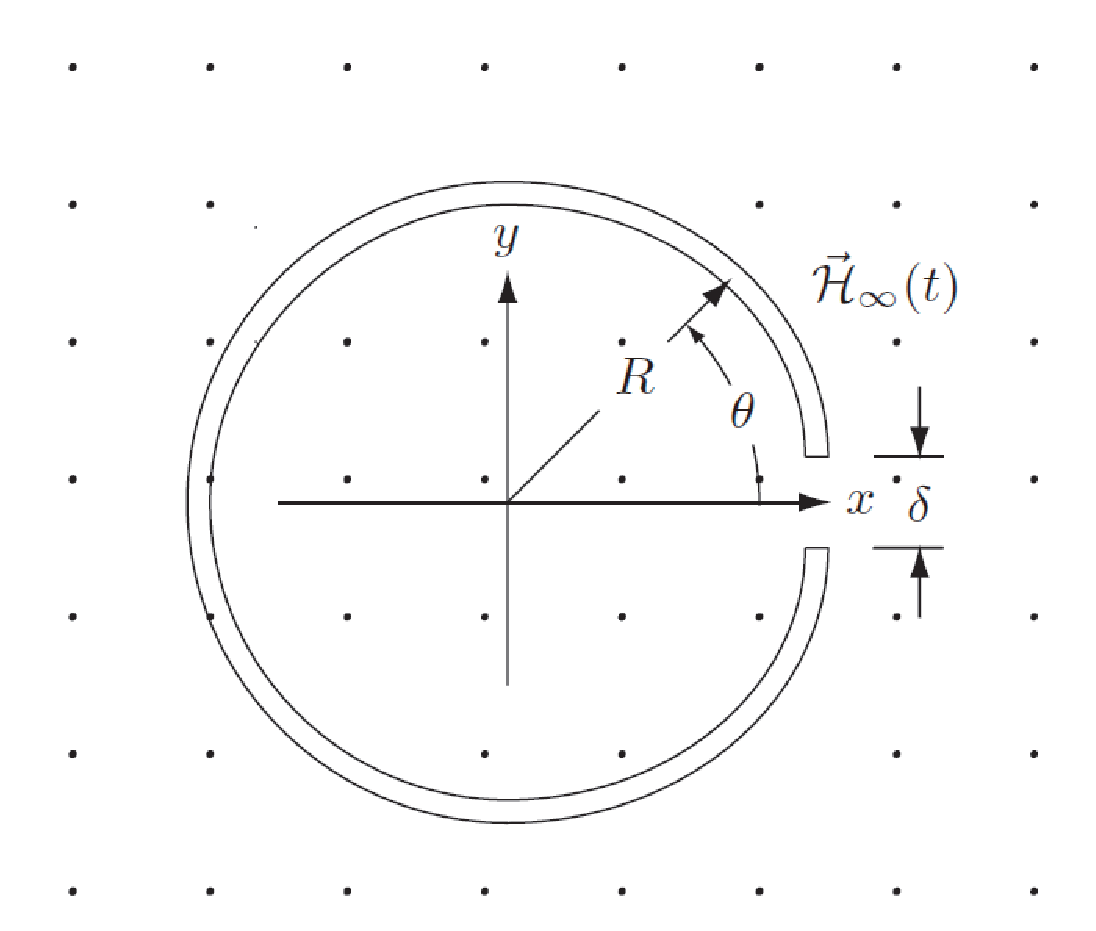
\includegraphics[scale=0.4]{chpt2/figs/fig2.9.eps}
  \caption{置于z向正弦时变磁场的在$\theta=0$处有窄缝的半径为R的理想导体长薄圆柱体的轴向视图。}
\end{figure}

\subsubsection*{问题2.6之解}
a)对一阶电场$\vec{E}_1(t)$应用积分形式的Faraday定律:
\begin{equation*}
\CMcal{V}_1(t) \equiv \int_{C} \vec{E}_1 (t) \cdot d\vec{s}=-\pi R^2 \mu_0 \frac{d\CMcal{H}_0(t)}{dt}
\end{equation*}


线积分沿着圆柱逆时针进行(含窄缝)。上式右侧包括圆柱($\pi R^2$)所定义的整个区域。
因为圆柱是理想导体,故在材料内有$\vec{\mathcal{E}}_1(t)=0$。对线积分,仅有的非零贡献来自窄缝。以复幅值表示,有
$$V_{1|0}=-j\omega \pi R^2 \mu_0 H_0$$

b)应用Ohm定律,得到$J_1$(单位长度):
$$J_1=\frac{V_{1|0}}{\rho_s}$$

c)因为圆柱是理想导体。圆柱面上$\vec{E}_1$的切向分量必须为零。$\vec{E}_1$以直角离开或进入圆柱。
跨越圆柱的积分移动至窄缝左侧,积分区域减少,这令$|E_1|$变小。场线如图2.10所示。

d)这是c)的特例。从对称角度,可以准确计算出线积分。积分区域等于$\pi R^2/2$,即
$$V_1 |_{\theta=-\pi/2}^{\theta=+\pi/2}=-\frac{1}{2}j\omega \pi R^2 \mu_0 H_0$$

上式和a)表明,在同一轴向距离点,跨过圆柱的电压与电压触头方位有关。记住这一点,这在存在时变磁场(外施磁场,如本例;系统中电流产生的)条件下测电压时非常重要。
超导体交流损耗的电测法就是一个非常好的例子。

\begin{figure}
  \centering
 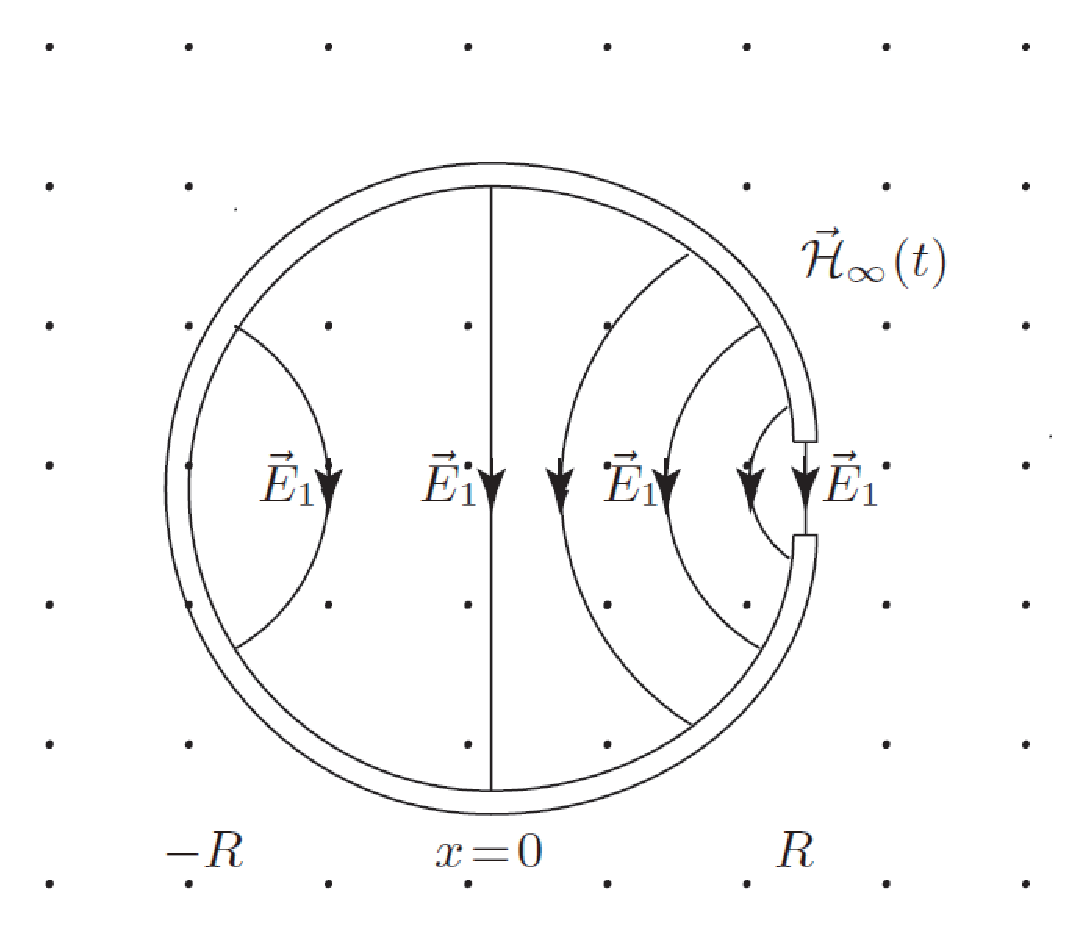
\includegraphics[scale=0.4]{chpt2/figs/fig2.10.eps}
  \caption{$\vec{E}_1$线垂直于理想导体圆柱。注意到,从$x=R$到$x=-R$,$|E_1|$是减小的。}
\end{figure}


\subsection{问题2.7:圆柱壳的感应加热}
本问题处理金属(非超导)圆柱壳的感应加热。它是一个同时涉及时谐电磁场、能流(Poynting矢量)、能量耗散的好例子。
本体和下一题是交流损耗,特别是涡流损耗的实例,本课题将在第七章进一步讨论。
感应加热在电炉中广泛使用,用以在导体材料内获得高温。有时,也用来作为研究超导线圈热行为的研究工具。
在超导磁体技术研究中,感应加热最常以脉冲场形式在其他超导线圈中产生小的正常区域,模拟暂态扰动。

图2.11给出一个“长”金属圆柱壳,其电导率为$\rho_e$,外径为$2R$,厚度$d\ll R$,置于正弦时变磁场中。磁场的0阶分量在z向均匀。即
$$\vec{\mathcal{H}}_\infty(t)=Re[H_0 e^{j\omega t}] \vec{i}_z$$
式中,$H_0$是复磁场幅值。

我们首先用两种方法解出相应的场量。接下来,用两种方法解出援助内的能量耗散。

\begin{figure}
  \centering
 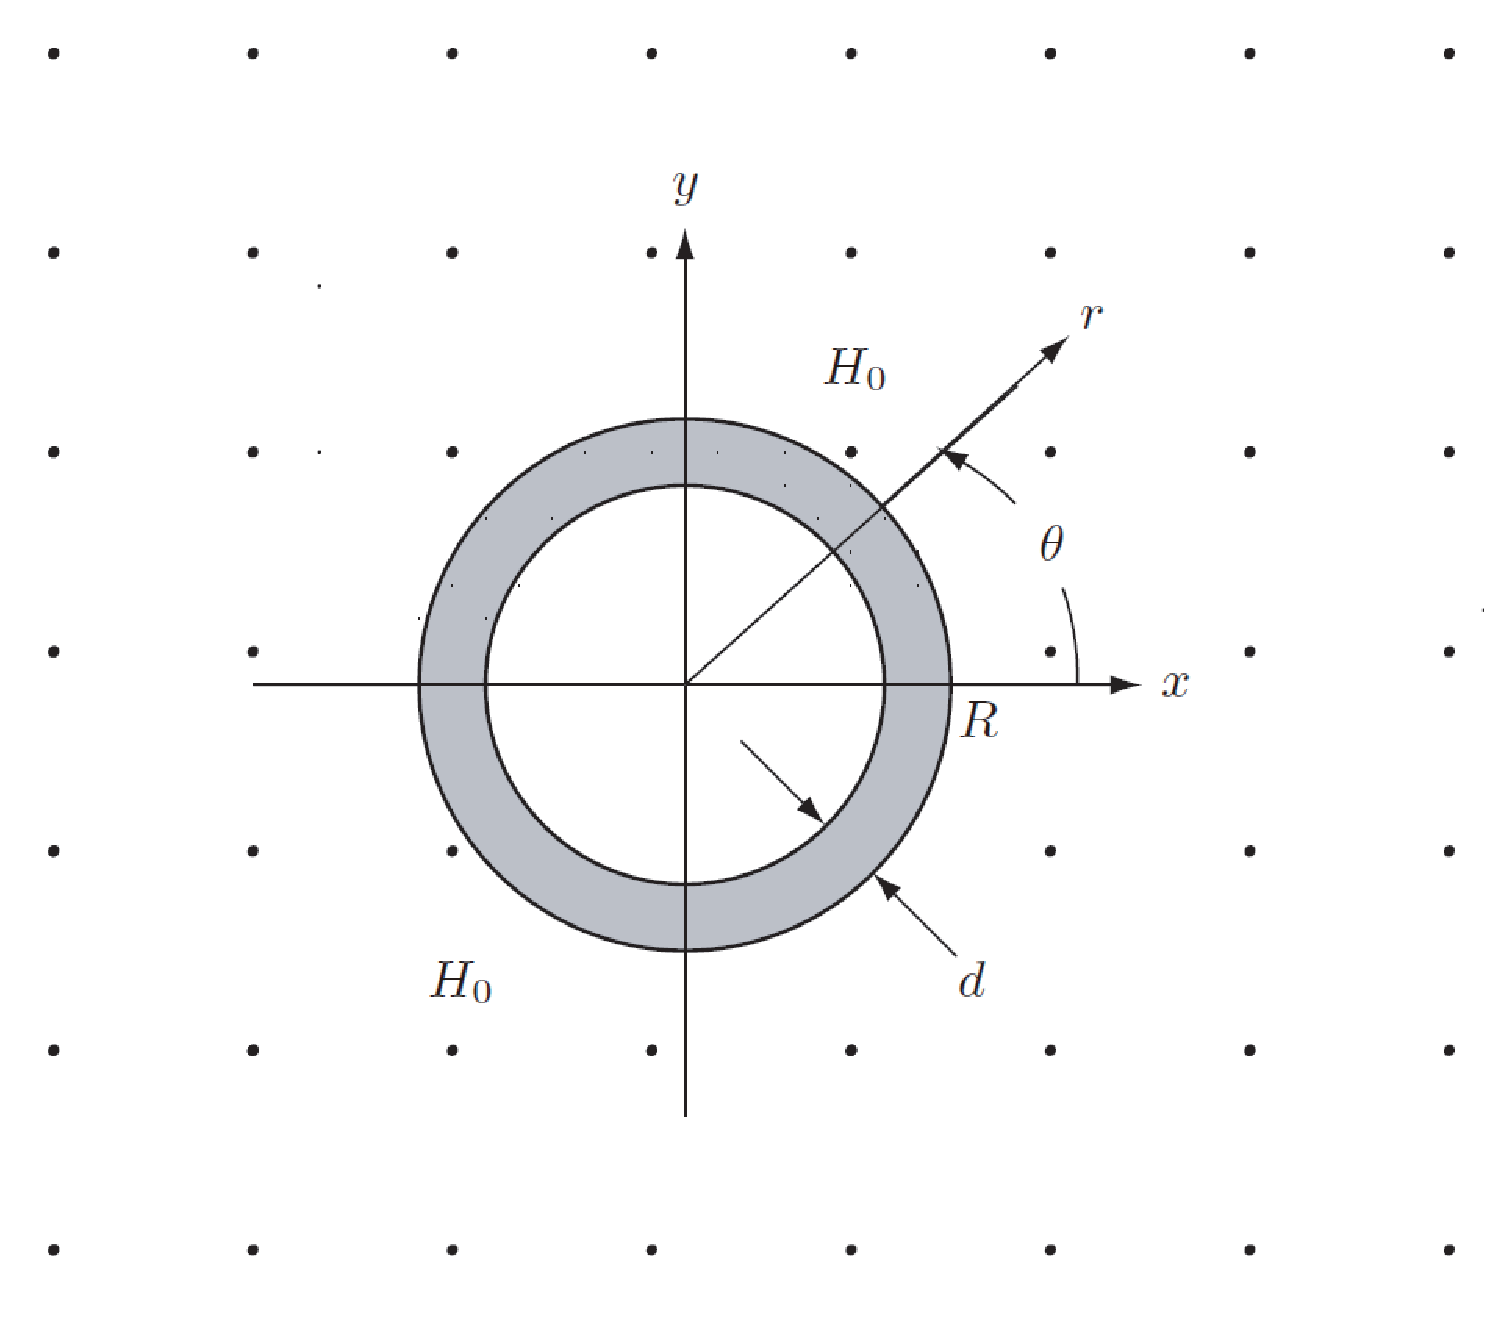
\includegraphics[scale=0.3]{chpt2/figs/fig2.11.eps}
  \caption{圆柱金属壳置于均匀正弦时变磁场之中。}
\end{figure}

\subsubsection*{第一部分:感应加热场的问题}
首先,用两种方法解出场量。

\textbf{方法一}

a)使用积分形式的Maxwell方程,忽略端部效应。证明在$r\le R$区域内给出一阶电场$\vec{E}_1$,在$r\simeq R$的壳内给出一阶电流密度$\vec{J}_1$的表达式为:
$$\vec{E}_1=-\frac{j\omega \mu_0 r H_0}{2} \vec{i}_\theta$$
$$\vec{J}_1=-\frac{j\omega \mu_0 R H_0}{2\rho_e} \vec{i}_\theta$$

b)证明:在$r\le R-d$区域,一阶磁场$\vec{H}_1$可以表示为
$$\vec{H}_1=-\frac{j\omega \mu_0 R d H_0}{2\rho_e} \vec{i}_z$$

c)上面三式,在准静态近似条件下得出,仅在“低”频下成立,或者说仅在频率远小于“趋肤深度”频率$f_{sk}$下成立。证明:
$$f_{sk}=\frac{\rho_e}{\pi \mu_0 R d}$$

\textbf{方法二}

方法一得到的$\vec{E}_1$、$\vec{J}_1$、$\vec{H}_1$均随着$\omega$增大,仅在频率小于$f_{sk}$时成立。下面,我们用一种新技术来推出在所有频率下均成立
的室温孔内场$\vec{H}_T=\vec{H}_0+\vec{H}_r$的完整表达式。式中,$\vec{H}_T$是总场,$\vec{H}_0$是原场,$\vec{H}_R$是室温孔内的系统反应场。

本方法中,首先将$\vec{H}_T=\vec{H}_0+\vec{H}_r$视为零阶场,解出作为一阶磁场响应的$\vec{H}_R$。

d)证明在$d\ll R$条件下壳内的$\vec{H}_R$、$\vec{H}_T$和$\vec{J}$为:
$$\vec{H}_R=-\frac{j\omega \mu_0 R d H_0}{2\rho_e+j\omega \mu_0 R d} \vec{i}_z$$
$$\vec{H}_T=\frac{2\rho_e H_0}{2\rho_e+j\omega \mu_0 R d} \vec{i}_z$$
$$\vec{J}=-\frac{j\omega \mu_0 R H_0}{2\rho_e+j\omega \mu_0 R d} \vec{i}_\theta$$

\subsubsection*{第一部分:感应加热场的问题之解}
根据$\theta$方向的对称性,$\vec{E}_1$和$\vec{J}_1$在$\theta$方向为常量,两个量均为$\theta$向,且仅依赖于r。这样,Faraday感应定律可在r的边线$\mathcal{C}$
上进行,围城的面积为$\mathcal{S}$:
$$\oint_{\mathcal{C}} \vec{E}_1 \cdot d\vec{s}=-j\omega \mu_0 \int_{\mathcal{S}} \vec{H}_0 \cdot d\vec{\mathcal{A}}$$
$$\int_{0}^{2\pi} r E_{1\theta} d\theta=-j\omega \mu_0 \int_{0}^{r} 2\pi r H_0 dr$$
$$E_{1\theta}\int_{0}^{2\pi} r d\theta=-j\omega \mu_0 H_0\int_{0}^{r} 2\pi r dr$$

在$r\le R$时
$$E_{1\theta} 2\pi r = -j\omega \mu_0 H_0 \pi r^2$$

上式两侧同除$2\pi r$,有
$$E_{1\theta} = -\frac{j\omega \mu_0 r H_0}{2}$$

于是
$$\vec{E_{1}} = -\frac{j\omega \mu_0 r H_0}{2}\vec{i}_\theta$$

一阶电流仅在壳内($r\simeq R$)流动
$$\vec{J}_1=\frac{\vec{E_{1}}(r\simeq R)}{\rho_e} = -\frac{j\omega \mu_0 R H_0}{2\rho_e}\vec{i}_\theta$$

在$d\ll R$时,我们可以将电流处理为一阶表面电流$\vec{K}_1$:
$$\vec{K}_1=\vec{J}_1 \cdot d= -\frac{j\omega \mu_0 R d H_0}{2\rho_e}\vec{i}_\theta$$

b)对$r>R$,$\vec{H}_1=0$;我们可以将上述面电流等效为在$r=R$处$\vec{H}$的不连续:壳内壁$\vec{H}_0+\vec{H}_1$,壳外$\vec{H}_0$。于是
$$\vec{K}_1=\vec{i}_r \times [\vec{H}_0-(\vec{H}_0+\vec{H}_1)]=-\frac{j\omega \mu_0 R d H_0}{2\rho_e}\vec{i}_\theta$$

在$d\ll R$条件下解出$\vec{H}_1(r\le R-d)$
$$\vec{H}_1=-\frac{j\omega \mu_0 R d H_0}{2\rho_e}\vec{i}_z$$

c)前已表明,$\vec{J}_1$、$\vec{K}_1$和$\vec{H}_1$的幅值均随着频率单调增长。这意味着它不可能在所有$\omega$下成立。
事实上,那些解仅在准静态近似可以应用的低频下有效。特别的,仅在$|\vec{H}_1|\ll |\vec{H}_0|$时有效:
$$|\vec{H}_1|=\frac{\omega \mu_0 R d |H_0|}{2\rho_e}\ll |\vec{H}_0|$$

由上式,可以得到频率极限,即通常所谓的趋肤深度频率$f_{sk}$。在此频率下,准静态近似是有效的
$$f_{sk}=\frac{\rho_e}{\pi \mu_0 R d}$$

注意,$f_{sk}$不仅与材料的电阻率有关,还与处于正弦时变磁场中的物体的尺寸有关。

d)在计算反应场时,设定$\vec{H}_1\equiv \vec{H}_R$。在$\vec{H}_1$的表达式中,用$\vec{H}_0+\vec{H}_R$代换$\vec{H}_0$
$$\vec{H}_R=-\frac{j\omega \mu_0 R d (\vec{H}_0+\vec{H}_R)}{2\rho_e}$$

解出$\vec{H}_R$,得到
$$\vec{H}_R=-\frac{j\omega \mu_0 R d \vec{H}_0}{2\rho_e+j\omega \mu_0 R d}\vec{i}_z$$

于是,可以得到
$$\vec{H}_T=\vec{H}_0+\vec{H}_R=\frac{2\rho_e H_0}{2\rho_e+j\omega \mu_0 R d}\vec{i}_z$$

$\vec{J}$和$\vec{H}_R$通过$\nabla\times \vec{H}=\vec{J}$相联系,又$\vec{K}=\vec{J}d$,于是
$$\vec{J}=\frac{1}{d}H_R \vec{i}_\theta=-\frac{j\omega \mu_0 R H_0)}{2\rho_e+j\omega \mu_0 R d}\vec{i}_\theta$$

注意到,在低频下,$\vec{H}_R$退化为$\vec{H}_1$;高频下,$\vec{H}_R$退化为$-\vec{H}_0$而$\vec{H}_T$变为0。$\vec{J}$存在类似的行为。

\subsubsection*{第二部分:感应加热的能量耗散}
我们用两种方法解出圆柱内的能量耗散。

\textbf{方法一}

e)我们可以直接计算$<p>=\vec{E}\cdot \vec{J}^* /2=\rho_e |J|^2 /2$而得到圆柱壳的电阻功率损耗。式中的$\vec{J}$已在前文求出。
证明:在$d\ll R$条件下,壳内的时均总损耗(单位长度)的表达式为
$$<P>=2\pi R d<p>=\frac{\pi \rho_e \omega^2 \mu_0^2 R^3 d}{4\rho_e^2+\omega^2\mu_)^2 R^2 d^2} |H_0|^2$$

\textbf{方法二}

相同的施于圆柱的复功率也可以视为从$r>R$处的源在$r=R$处进入圆柱内的Poynting能流。

f)证明:在$r=R$处,进入圆柱的一阶复Poynting矢量$\vec{S}_1$的面积分(单位长度)为:
$$-\oint_{\mathcal{S}}\vec{S}_1 \cdot d\mathcal{A}=\frac{1}{2}(2\pi P)E_{1\theta} H_)^*$$

提示:$E_{1\theta}=\rho_e J_\theta$,$J_\theta$已在上文求出。

g)证明:上式的等号右侧的实部与e)中给出的$<P>$是一致的。

h)画出$<P>$与$\rho_e$的关系。由于理想导体($\rho_e=0$)和理想绝缘体($\rho_e=\infty$)均不产生损耗,图像应从$<P>=0$开始,并在$\rho_e \rightarrow \infty$时趋于0。

i)从$<P>$与$\rho_e$的关系可以得到一个结论,即存在临界电阻率$\rho_{e_c}$,在该点$<P>$最大。证明
$$\rho_{e_c}=\frac{\omega \mu_0 R d}{2}$$

从上式可知,对一个电阻率($\rho_e$)和样品尺寸($R,d$)组合,存在一个可以令加热最大化的最优频率。这个频率就是前面提到的趋肤深度频率$f_{sk}$。

j)计算一个半径$R=10mm$,壁厚$d=0.5mm$,电阻率$\rho_e=2\times 10^{-10} \Omega\cdot m$(大致为液氦温度下铜的电阻率)的铜管的$f_{sk}$。

\subsubsection*{第二部分:感应加热的能量耗散之解}
e)正弦情况下,时均能耗(单位长度)功率可以表示为$<p>=\vec{E}\cdot \vec{J}^* /2=\rho_e |J|^2 /2$,也即
$$<p>=\rho_e |J|^2 /2=\frac{\rho_e}{2}(\frac{\omega^2 \mu_0^2 R^2}{4\rho_e^2+\omega^2 \mu_0^2 R^2 d^2})|H_0|^2$$

于是,壳内总的能耗(单位长度)可以能耗功率乘以截面积得到
$$<P>=2\pi R d<P>=\frac{\pi \rho_e \omega^2 \mu_0^2 R^3 d}{4\rho_e^2+\omega^2 \mu_0^2 R^2 d^2}|H_0|^2$$

下面检查一下上式在$\rho_e$两个极限下的情况:
\begin{itemize}
  \item $\rho_e \ll \omega \mu_0 R d$(良导体)时:$<P>\simeq \frac{\pi \rho_e R}{d}|H_0|^2\propto \rho_e$
  \item $\rho_e \gg \omega \mu_0 R d$(不良导体)时:$<P>\simeq \frac{\pi \omega^2 \mu_0^2 R^3 d}{4\rho_e}|H_0|^2\propto \frac{1}{\rho_e}$
\end{itemize}

正如我们所期望的,在上面两种极限情况下,都有$<P>\rightarrow 0$。

f)复Poynting矢量$\vec{S}$的一阶展开为:
$$\vec{S}_1=\frac{1}{2}(\vec{E}_0 \times \vec{H}_0^*+\vec{E}_0 \times \vec{H}_1^*+\vec{E}_1 \times \vec{H}_0^*)$$

计算一阶Poynting矢量时,E和H场的下表均不大于1。在本例下,我们有$\vec{E}_)=0$,于是上式化简为:
$$\vec{S}_1=\frac{1}{2}(\vec{E}_1 \times \vec{H}_0^*)$$

对于$\vec{E}_1$我们有:
$$\vec{E}_1=\rho_e \vec{J}=-\frac{j\rho_e \omega \mu_0 R H_0)}{2\rho_e+j\omega \mu_0 R d}\vec{i}_\theta$$

于是,
$$-\oint_{\mathcal{S}}\vec{S}_1 \cdot d\mathcal{A}=\frac{1}{2}(2\pi R)E_{1\theta} H_0^*=\frac{j\pi\rho_e \omega \mu_0 R^2}{2\rho_e+j\omega \mu_0 R d} |H_0|^2$$

g)根据复数的基本运算法则,取f)最后结果的实部,易得。可以看到,这和方法一得到的结果是一致的。

h)如图2.12所示。

i)将$<P>$对$\rho_e$求导,并令之为零,有:
$$\frac{d<P>}{d\rho_e} |_{\rho_{e_c}}=[**]=0$$

解出上式,有
$$\rho_{e_c}=\frac{\omega \mu_0 R d}{2}$$

上式在均匀正弦时变磁场施加于导体样品的感应加热应用中非常重要。样品被样品中感应的涡流加热。在趋肤深度频率$f_{sk}$下,感应加热最大。

j)将数值$R=1cm, d=0.5mm,\rho_e=2\times 10^{-10}\Omega m$(4K时铜的电阻率)代入公式,有
$$f_{sk}=\frac{\rho_{e_c}}{\pi\mu_0 R d}\simeq 10Hz$$

\begin{figure}
  \centering
 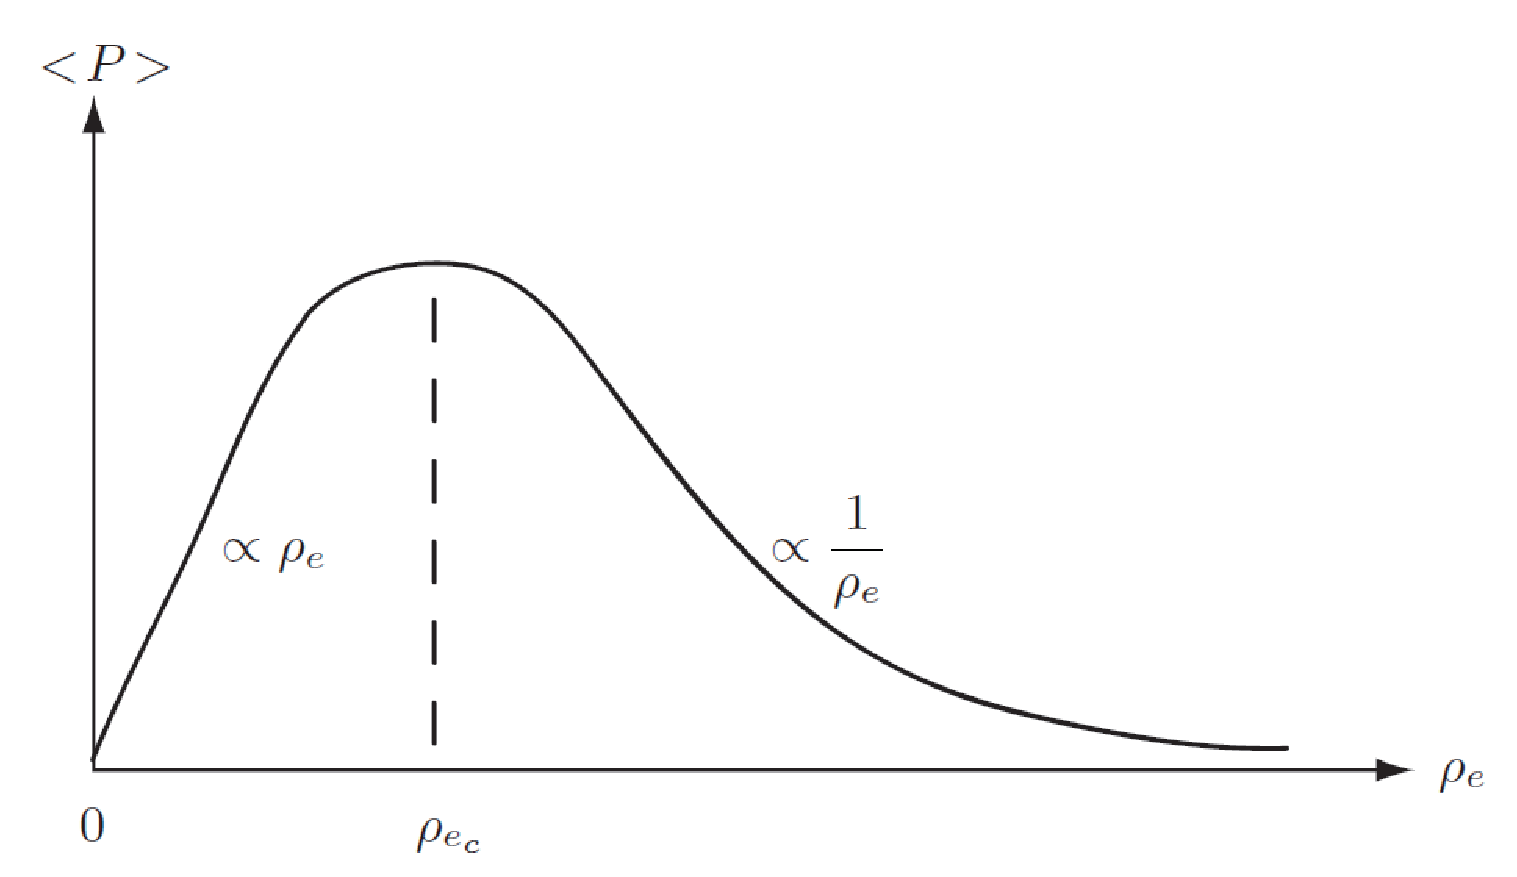
\includegraphics[scale=0.3]{chpt2/figs/fig2.12.eps}
  \caption{感应加热圆柱壳的功率耗散和电阻率的关系。}
\end{figure}


\subsection{问题2.8:金属窄带中的涡流损耗}
本题推导置于时变磁场中的金属窄带的涡流损耗。这可以用于计算铜基超导带中涡流损耗的计算。(感应电流有用时叫感应加热,有害时就叫涡流损耗。)

图2.13给出了电导率为$\rho_e$、y向宽为b、厚度(z向)为a的长(x向)金属窄带。窄带置于时变外磁场中。外场满足$dB_0/dt=\dot{B_0}$,即零阶、均匀、z向。

a)证明一阶电场$\vec{E}_1$为
$$E_{1x}=y\dot{B_0}$$

b)证明空间平均能耗密度$\tilde{p}$(单位体积)为:
$$\tilde{p}=\frac{(b\dot{B_0})^2}{12\rho_e}$$

c)外场以角频率$\omega$正弦变化,即$B(t)=B_0 \sin\omega t$时,证明:时均能耗密度为:
$$<\tilde{p}>=\frac{(b\omega\dot{B_0})^2}{24\rho_e}$$

\begin{figure}
  \centering
 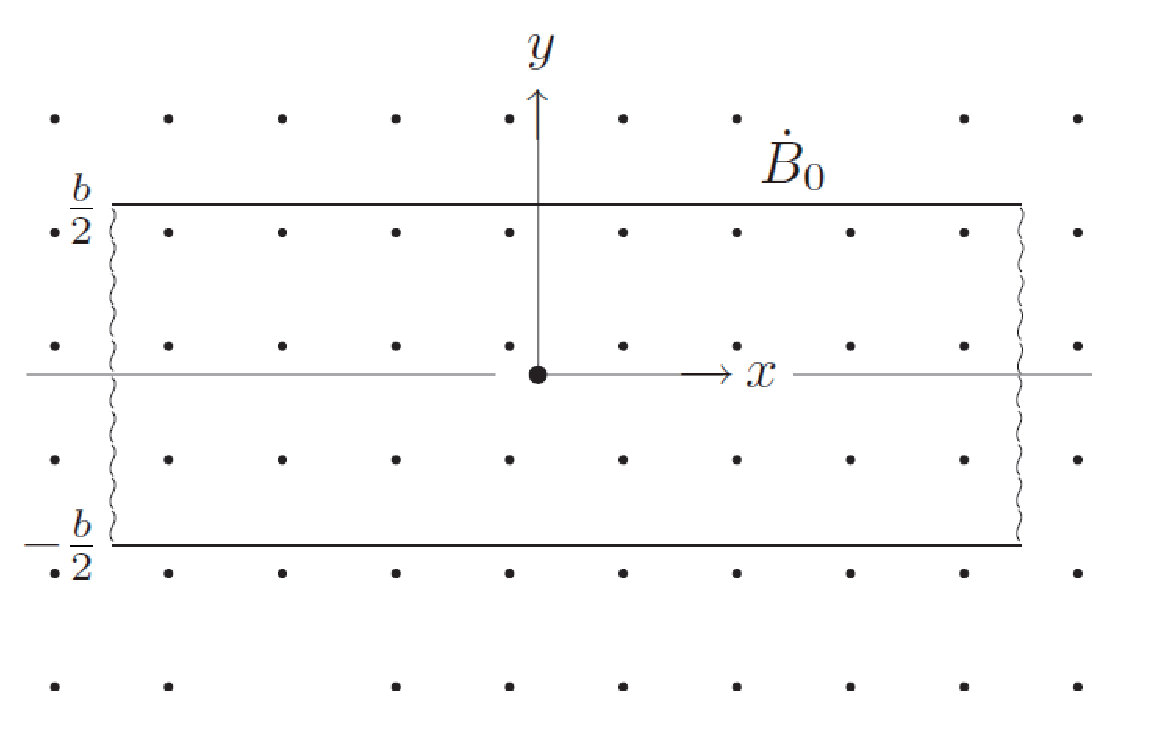
\includegraphics[scale=0.4]{chpt2/figs/fig2.13.eps}
  \caption{宽度为b的金属窄带置于时变磁场中。}
\end{figure}

\subsubsection{问题2.8之解}
a)由于$\vec{B}_0$时均匀分布的且系统不依赖于x,所以$\vec{E}_1$只能指向x方向并且仅依赖于y。于是$\nabla\times \vec{E}_1=\partial \vec{B}_0/\partial t$可以化简为
$$-\frac{dE_{1x}}{dy}=-\frac{B_0}{dt}=-\dot{B}_0$$

根据对称性,$E_{1x}(y=0)=0$,于是,我们有
$$E_{1x}=y\dot{B_0}$$

b)窄带中的局部能量损耗密度$p(y)$由$\vec{E}_1\cdot\vec{J}_1$给出。总的损耗(单位长度)为
$$P=a\int_{-b/2}^{b/2}p(y)dy=\frac{2a(\dot{B}_0)^2}{\rho_e}\int_{0}^{b/2}y^2dy=\frac{ab(b\dot{B_0})^2}{12\rho_e}$$

上式仅在$\vec{J}_1$感应出来的一阶感应磁场相比$\vec{B}_0$很小时才有效。

空间平均能耗密度$\tilde{p}$(单位体积)可以由P除以截面得到:
$$\tilde{p}=\frac{P}{ab}\frac{(b\dot{B_0})^2}{12\rho_e}$$

c)在外场正弦变化时,时均能耗密度为:
$$<\tilde{p}>=\frac{1}{2}E_{1x} J_{1x}^*$$

由于$E_{1x}=j\omega y B_0$,$J_{1x}=E_{1x}/\rho_e$,于是可以得到
$$<\tilde{p}>=\frac{2a(\omega B_0)^2}{2\rho_e (ab)}\int_{0}^{b/2} y^2 dy=\frac{(b\omega\dot{B_0})^2}{24\rho_e}$$

我们注意到,$\tilde{p}$和$<\tilde{p}>$分别正比于$(b\dot{B_0})^2$和$(b\omega \dot{B_0})^2$。也就是说,两者对感应磁场和导体宽度均为平方依赖关系。

\subsection{讨论2.4:分层以减少涡流损耗}
假设将薄板劈为两条,每一条宽度为$b/2$,由上面的分析可以知道,损耗将变为原来的$1/4$。因此,可以通过将窄带细分的方法降低涡流损耗。这种切分技术在电力变压器中广泛使用。类似的,我们将在第5章和第7章中看到,超导体也能从切分中获益。


\subsection{问题9:Rogowski线圈}
Rogowski线圈是时变电流的安培计。它是一种环形拾磁线圈,其积分输出电压正比于被线圈包围的截面内通过的总电流。图2.14a给出了一个Rogowski线圈,待测电流$I(t)$置于其中央。如图所示,Rogowski线圈包括N个串联的小圆环(一匝)。每一个半径为c的圆环的中心位于电流中心的径向R处。
图2.14b定义了一匝的x-y坐标。

a) 证明在$c\ll R$条件下,N匝的Rogowski线圈的总磁链$\Phi(t)=N\Phi_1(t)$为:
$$\Phi(t)\simeq\frac{\mu_0 N c^2}{2R}I(t)$$
式中,$\Phi_1(t)$是与一匝交链的总磁通。

b) 证明$\Phi(t)$的准确表达式为:
$$\Phi(t)=\mu_0 N (R-\sqrt{R^2-c^2})I(t)$$

将N匝中的一个放在x-y坐标系的中心来计算$\Phi(t)$。

c) 证明在极限$(c/R)^4\ll 1$下,b)退化为a)。

d)证明b)中的公式在Rogowski线圈的轴线偏离电流的中心时也有效。

e)计算一个N = 3600; c = 3 mm; R = 0.5 m的Rogowski线圈在$\Delta I(t)=1MA$时两端产生的伏秒。

\begin{figure}
  \centering
 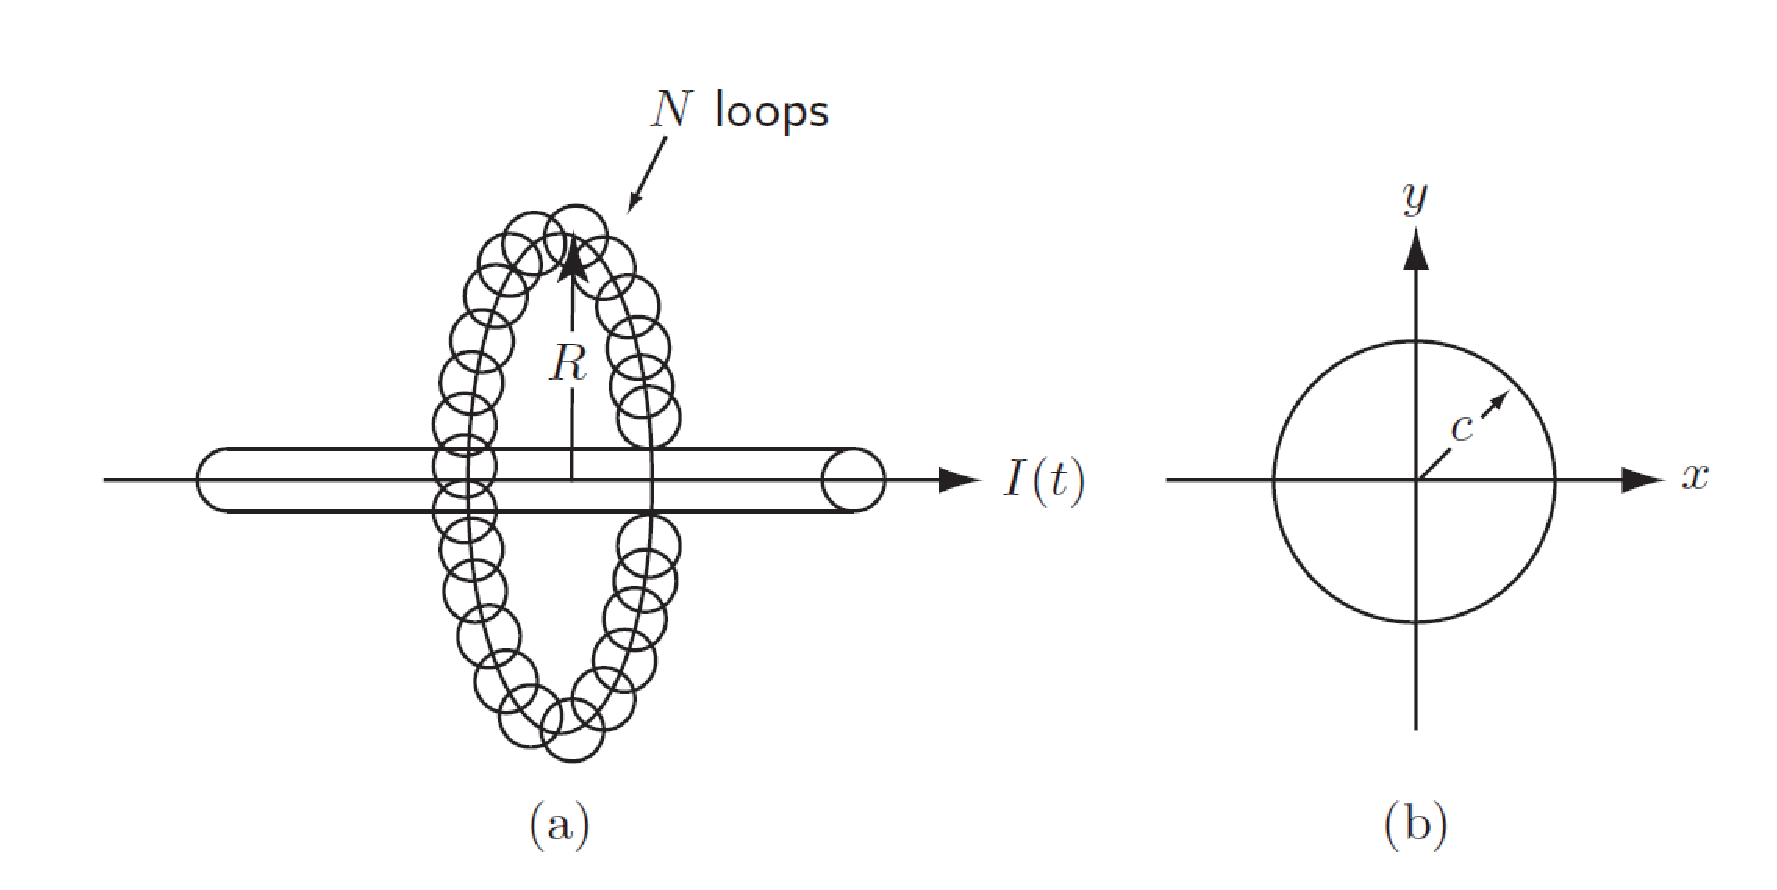
\includegraphics[scale=0.4]{chpt2/figs/fig2.14.eps}
  \caption{(a)N匝Rogowski线圈,每匝直径为2c,环绕在待测的时变电流$I(t)$外围。(b)一匝(半径为$r$)的截面视图。圆环距离电流中心的距离为$R$。}
\end{figure}

\subsubsection{问题13之解}
a)电流$I(t)$产生的磁场相对于电流方向是方位角向的。距电流中心距离R处的$H_\phi(t)$表示为:
$$H_\phi (t)=\frac{I(t)}{2\pi R}$$

对于$c\ll R$,上式给出的$H_\phi(t)$在每一匝的横截面$\pi c^2$上几乎都是成立的。由于Rogowski线圈有$N$个这样的回路,我们有:
$$\Phi(t)\simeq \frac{\mu_0 N c^2}{2R}I(t)$$

Rogowski线圈输出电压$V(t)$于是可以写为:
$$V(t)=\frac{d\Phi(t0}{dt}=\frac{\mu_0 N c^2}{2R}\frac{dI(t)}{dt}$$

b)因为$H_\phi (t)$在每一个环上并非常数,每一匝包围的总磁通$\Phi_1(t)$应由沿回路围成的区域的积分得到。
注意到$x^2+y^2=c^2$,定回路中心坐标为$(0,0)$,$\Phi_1(t)$表示为:
$$\Phi (t)=\frac{\mu_0 I(t)}{2\pi}\int_{-c}^{c}\int_{-\sqrt{c^2-y^2}}^{\sqrt{c^2-y^2}}\frac{1}{R+y}dxdy=\frac{\mu_0 I(t)}{\pi}\int_{-c}^{c}\frac{\sqrt{c^2-y^2}}{R+y}dy$$

上式可以使用新变量$\xi\equiv R+y$得到闭式解(注意:$d\xi=dy$)。于是,有:
$$\Phi_1 (t)=\frac{\mu_0 I(t)}{\pi} \int_{R-c}^{R+c}\frac{\sqrt{c^2-R^2+2R\xi-\xi^2}}{\xi}d\xi=\mu_0(R-\sqrt{R^2-c^2})I(t)$$

$N$匝的Rogowski线圈交链的总磁通$\Phi(t)=N\Phi_1(t)$:
$$\Phi (t)=\mu_0 N(R-\sqrt{R^2-c^2})I(t)$$

c)上式可以写为:
$$\Phi (t)=\mu_0 NI(t)(R-R\sqrt{1-\frac{c^2}{R^2}})$$

由于对$x\ll 1$,$\sqrt{1-x}\simeq 1-(1/2)x+(1/8)x^2-...$,截取到二阶,所以
$$\Phi (t)\simeq \frac{\mu_0 Nc^2}{2R} I(t)\eqno{(2.69)}$$

\begin{figure}
	\centering
	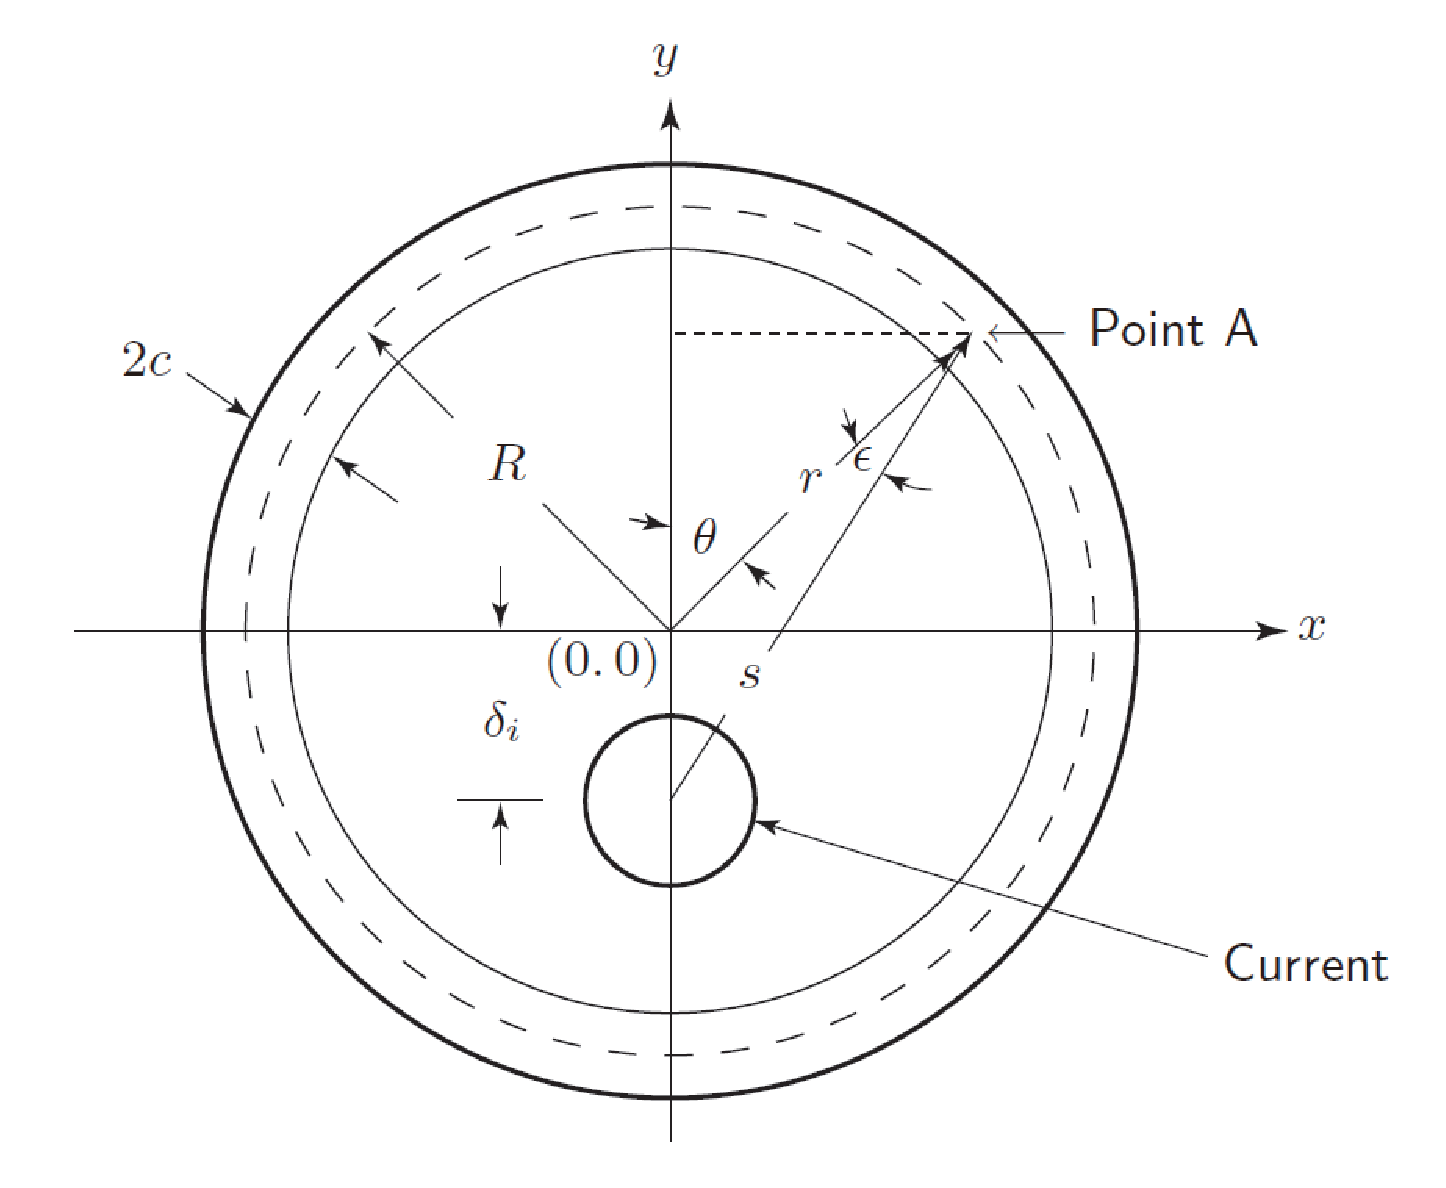
\includegraphics[scale=0.4]{chpt2/figs/fig2.15.eps}
	\caption{$(x,y)$面上的横截面视图}
\end{figure}

d)图2.15给出正交于电流/Rogowski线圈组方向的横截面$(x,y)$,其中Rogowski中心位于$(0,0)$,电流中心在Rogowski线圈中心向下偏离$\delta_i$。关键参数如图中定义:$r$,Rogowski中心$(0,0)$到一匝线圈上的点A的径向距离;$\theta$是$y$轴和$r$之间的夹角;$s$是电流中心到点A的距离;$\epsilon$是$r$与$s$之间形成的角。$s^2$写为:
$$s^2=(r\cos\theta+\delta_i)^2+r^2\sin^2\theta=r^2+\delta_i^2+2r\delta_i\cos\theta$$

将$r$延长$\delta_i \cos\theta$形成一个直角,我们有:
$$\cos\epsilon=\frac{r+\delta_i \cos\theta}{s}$$

点A处的磁场由$H_A(t)=I(t)/2\pi s$给出;它在Rogowski线圈回路上点A处的法向分量为:
$$H_{A\bot}=\frac{I(t)}{2\pi s}\cos\epsilon=\frac{I(t)}{2\pi s}(\frac{r+\delta_i \cos\theta}{s})$$

将上式与$s^2$的表达式联立,得到:
$$H_{A\bot}=\frac{I(t)}{2\pi}\left(\frac{r+\delta_i \cos\theta}{r^2+\delta_i^2+2r\delta_i\cos\theta}\right)\eqno{(S9.10)}$$

为了计算$\Phi(t)$,$S9.10$乘上$(N/2\pi)2\sqrt{c^2−(r−R)^2}$必须积分两次:第一次对$\theta$从$0$至$2\pi$积分,视径向距离$r$为常数,计及$N$匝;第二次对$R$从$R-c$到$R+c$积分。注意到$2\sqrt{c^2−(r−R)^2}$是每一匝直径为$c$的线圈在$r$处总的弦距离(z向),它位于距离回路中心的$r-R$处。
$$\Phi(t)=\frac{N I(t)}{2\pi^2}\int_{R-c}^{R+c}\int_{0}^{1\pi}\left[ \frac{(r+\delta_i \cos\theta)\sqrt{c^2-(r-R)^2}}{r^2+\delta_i^2+2r\delta_i \cos\theta}\right]d\theta dr\eqno{(S9.11a)}$$

$$=\frac{N I(t)}{\pi}\int_{R-c}^{R+c} \left[ 0+\frac{\sqrt{c^2-(r-R)^2}}{r}\right]dr\eqno{(S9.11b)}$$

注意到积分中完全没有$\delta_i$。下面,$S9.11b$沿着一匝的径向从$r=R-c$到$r=R+c$积分,有:
$$\Phi(t)=\frac{N I(t)}{\pi}\left[ \pi(R-\sqrt{R^2-c^2})\right]$$

可见,Rogowski线圈可以精确的测量电流$I(t)$,不管它与其套入的电流是否同心。

e) 对于$N = 3600, c = 3 mm; R = 0.5 m; \Delta I = 1 MA$,公式2.69可以应用,因为$(c/R)^4 = 1.3×10^{−9}\ll 1$。这样,由$S9.2$得:
$$\int V(t)dt=\frac{\mu_0 N c^2 \Delta I}{2R}\simeq 41 mVs$$

在一个噪音环境中,比如典型的试验聚变机器中,测到$40 mVs$级别的信号水平并不简单,但也不是完全得不到。

\begin{quotation}
\kaishu 正如我们所知,有已知的已知,他们是我们知道我们知道的;我们也知道有些是已知的未知。这就是说我们知道有些事情我们是不知道的。但是还有未知的未知——这些事我们不知道我们不知道。——Donald Rumsfeld,2002
\end{quotation}